
\chapter{Introduction}

OpenSCHC offers an easy way to understand and experiment the compression/decompression mechanism as well as the fragmentation protocol. OpenSCHC does not require to run on a LPWAN network, experiments can run on a regular network.


\chapter{Installation}\label{chap-plat}

\section{Download code}

To download openSCHC, just clone the openschc repository on github.


\begin{lstlisting}
> git clone git@github.com:openschc/openschc.git
\end{lstlisting}

and use the scapy branch.

\begin{lstlisting}
> git checkout scapy
\end{lstlisting}

\section{Setup the environment}

For testing SCHC, we are going to generate some IPv6 packets, that will be caught by scapy and processed. 

~

An IPv6 prefix is needed for that traffic. A simple way to get a global IPv6 prefix is to use Hurricane Electric tunnel broker:
\begin{itemize}
\item Go to that website \url{https://tunnelbroker.net/}, 
\item Create an account if needed or just log in, 
\item Select \textit{Create another Tunnel},
\item enter the IPv4 address of the machine running openSCHC and a location,
\end{itemize}

Once the tunnel created, you will find some configuration examples, that will help you to configure your machine.

For ubuntu 20, it will be in the /etc/netplan directory:

\begin{lstlisting}
> cat /etc/netplan/50-cloud-init.yaml
# This file is generated from information provided by
# the datasource.  Changes to it will not persist across an instance.
# To disable cloud-init's network configuration capabilities, write a file
# /etc/cloud/cloud.cfg.d/99-disable-network-config.cfg with the following:
# network: {config: disabled}
network:
    ethernets:
        ens3:
            dhcp4: true
            match:
                macaddress: fa:16:3e:e9:db:5d
            addresses:
            - "2001:41d0:404:200:0:0:0:3a86/64"
            gateway6: "2001:41d0:0404:0200:0000:0000:0000:0001"
            set-name: ens3
    version: 2
    tunnels:
      he-ipv6:
       mode: sit
       remote: 216.66.87.102
       local: 51.91.121.182
       addresses:
         - "2001:470:1f20:1d2::2/64"
       gateway6: "2001:470:1f20:1d2::1"
\end{lstlisting}

and your machine interfaces looks the following:

\begin{lstlisting}
> ifconfig
ens3: flags=4163<UP,BROADCAST,RUNNING,MULTICAST>  mtu 1500
        inet 51.91.121.182  netmask 255.255.255.255  broadcast 0.0.0.0
        inet6 2001:41d0:404:200::3a86  prefixlen 64  scopeid 0x0<global>
        inet6 fe80::f816:3eff:fee9:db5d  prefixlen 64  scopeid 0x20<link>
        ether fa:16:3e:e9:db:5d  txqueuelen 1000  (Ethernet)
        RX packets 9543878  bytes 1758163442 (1.7 GB)
        RX errors 0  dropped 0  overruns 0  frame 0
        TX packets 9253880  bytes 1479370777 (1.4 GB)
        TX errors 0  dropped 0 overruns 0  carrier 0  collisions 0

he-ipv6: flags=209<UP,POINTOPOINT,RUNNING,NOARP>  mtu 1480
        inet6 fe80::335b:79b6  prefixlen 64  scopeid 0x20<link>
        inet6 2001:470:1f20:1d2::2  prefixlen 64  scopeid 0x0<global>
        sit  txqueuelen 1000  (IPv6-in-IPv4)
        RX packets 782095  bytes 447475094 (447.4 MB)
        RX errors 0  dropped 0  overruns 0  frame 0
        TX packets 71534  bytes 6022694 (6.0 MB)
        TX errors 5  dropped 0 overruns 0  carrier 5  collisions 0

lo: flags=73<UP,LOOPBACK,RUNNING>  mtu 65536
        inet 127.0.0.1  netmask 255.0.0.0
        inet6 ::1  prefixlen 128  scopeid 0x10<host>
        loop  txqueuelen 1000  (Local Loopback)
        RX packets 7212  bytes 657864 (657.8 KB)
        RX errors 0  dropped 0  overruns 0  frame 0
        TX packets 7212  bytes 657864 (657.8 KB)
        TX errors 0  dropped 0 overruns 0  carrier 0  collisions 0
\end{lstlisting}

Note that the machine is multi-homed; \texttt{ens3} interface is configured with the regular IPv6 address and \texttt{he-ipv6} with the Hurricane Electric IPv6 address. 

\section{Network Topology}

We have currently configured the network for the code part of SCHC. SCHC sends SCHC packet to another device which will also run SCHC. On that second machine, install the github repository, too.

~

With openSCHC the following topology (cf~\vref{fig-topo}) will be used for the rest of the tutorial. SCHC packet will be tunneled over the Internet to reach the other SCHC instance. 

 \begin{figure}[!ht] 
\centering 


	\begin{tikzpicture}[scale=0.8, transform shape]

	\draw (0,0) node(SCHC)[rectangle, minimum size=2cm, draw]{}; 
	\draw(SCHC) node {\small{SCHC}};
	\draw(SCHC.north) node [above]{\small{Core}};
	
	\draw(SCHC.south) -- ++(0, -1) coordinate(a);
	\draw (a) -- ++(-2, 0);
	\draw (a) -- ++(2, 0);
	
	\path (SCHC) -- ++(5, 3) coordinate (HE);
	
	\draw (HE) node [cloud, minimum width=3cm, minimum height= 2cm, draw] {};
	\draw [double, dashed] (HE) to [bend left=45] node [above, sloped] {IPv6} (SCHC);
	
	\path (SCHC) -- ++(-7, 0) coordinate (dev);
	\draw (dev) node(SCHC_dev)[rectangle, minimum size=2cm, draw]{}; 
	\draw(dev) node {\small{SCHC}};
	\draw (dev) node[cloud, minimum size=4cm, draw]{}; 
	\draw (SCHC_dev.north) node [above] {\small{Device}};
	
	
	\draw [very thick] (dev.south) to [bend right=80] node [below, sloped] {UDP}  node [above, sloped] {SCHC packet} (SCHC.south);
	
	

	\end{tikzpicture}
\caption{Network Topology} 
\label{fig-topo} 
\end{figure} 



\chapter{Rules}

SCHC  works between two entities. Usually, one is a constrained end-device and the other one is a core equipment acting as a router. To allow both of them to perform the same actions, or more precisely one action and a reverse action, such as compression and decompression or fragmentation and reassembly, a common set of rules must be shared between these two entities.

~

The distinction between a device and a core allows to differentiate communication going upstream from the device to the core and downstream in the opposite direction. The device usually owns a limited number of rules corresponding to the traffic  generated and received by that device. On the contrary, the core instance of SCHC must be aware of all the devices' rules. Even if all the devices have the same behavior, SCHC treats each device individually. 

~~

All rules are identified by a rule ID. The rule ID is a unique binary sequence for an association between a device and a core. The rule ID length is not specified and may be different inside a set of rule. The only constraint it that they cannot overlap.

For instance:


\begin{itemize}
\item\texttt{0} and \texttt{111111} are two valid rules ID
\item \texttt{01} and \texttt{0101} not not valid since they share the same first two bits.
\end{itemize}

~


Rules may be represented in binary, but the decimal notation is also used for compactness. In this book, we will represent a rule ID with the rule ID value/rule ID length. For instance \texttt{3/8} indicates a rule ID stored on 8 bits with value 3.

~

This notation can be misleading, if \texttt{1/2} and \texttt{127/7} taken from the example above are overlapping, \texttt{12/4} and \texttt{12/6} are two valuable rules, since they are written in binary \texttt{1100} and \texttt{001100} and do not share a common binary sequence.

~~~

In openSCHC, a rule is defined in a JSON object:

\begin{lstlisting}[backgroundcolor=\color{yellow}]
    {
    "RuleID" : 12,
    "RuleIDLength" : 4
    }
\end{lstlisting}

There is two different rule formats, one for compression and the other for fragmentation. Compression Rules contains the keyword \texttt{Compression} followed by an array, as shown the the minimal example bellow: 

\begin{lstlisting}[backgroundcolor=\color{yellow}]
   {
   "RuleID" : 12,
   "RuleIDLength" : 4,
   "Compression" : []
   }
   
\end{lstlisting}

   
Fragmentation rules uses the \texttt{Fragmentation} keyword followed by an object giving fragmentation parameters:

\begin{lstlisting}[backgroundcolor=\color{yellow}]
    {
    "RuleID" : 12,
    "RuleIDLength" : 4,
    "Fragmentation" : {
      "FRMode" : "NoAck",
      "FRDirection" : "UP"
    }
}
\end{lstlisting}

Fragmentation and compression rules share the same rule space, by construction a rule cannot be both compression and fragmentation. 
An attentive reader may have also noticed that a fragmentation direction is present in the rule description. 
In fact, compression rules are bi-directionnal and may be used to compress an header by the device and the core, but fragmentation rules are oriented.  

Finally a \texttt{NoCompression} keyword also exists and is the equivalent to the above example, indicating an uncompressed packet.

\begin{lstlisting}[backgroundcolor=\color{yellow}]
   {
   "RuleID" : 666,
   "RuleIDLength" : 10,
   "NoCompression" : []
   }
\end{lstlisting}


\section{Rule Manager}

The rule manager plays an important role in openSCHC. It has different goals:
\begin{itemize}
    \item check the rule correctness
    \item add default parameters
    \item display rules in a more synthetic format
    \item find the best rule to compress or fragment a packet
    \item find a rule from its rule ID.
\end{itemize}


\subsection{Rule definition}

The above listing gives a simple python program used to manage the two rules we described before. 


\begin{lstlisting}[language=Python]
from gen_rulemanager import *

RM = RuleManager()

rule1100 =   {
  "RuleID" : 12,
  "RuleIDLength" : 4,
  "Compression" : []
}

rule001100 =   {
  "RuleID" : 12,
  "RuleIDLength" : 6,
  "Fragmentation" :  {
    "FRMode" : "noAck",
    "FRDirection" : "UP"
  }
}

RM.Add(dev_info=rule1100)
RM.Add(dev_info=rule001100)

RM.Print()
\end{lstlisting}

~~


OpenSCHC displays:

\begin{lstlisting}[ basicstyle=\ttfamily\tiny]
****************************************
Device: None
/-------------------------\
|Rule 12/4          1100  |
|---------------+---+--+--+------------------------------+-------------+----------------\
\---------------+---+--+--+------------------------------+-------------+----------------/
/-------------------------\
|Rule 12/6        001100  |
!=========================+=============================================================\
!^ Fragmentation mode : noAck    header dtag 2 Window  0 FCN  3                     UP ^!
!^ No Tile size specified                                                              ^!
!^ RCS Algorithm: crc32                                                                ^!
\=======================================================================================/
\end{lstlisting}

Compression rules contain the field descriptions (here absent) and Fragmentation rules contain the fragmentation parameters. The rule manager added some default parameters corresponding to noAck behavior.


\subsection{Set of rules}

A device should contain a set of rules related to compression and fragmentation. In OpenSCHC, the SoR (Set of Rules) is a JSON array. The following program has the same behavior as the previous one.:

\begin{lstlisting}[language=Python]
from gen_rulemanager import *

RM = RuleManager()

rule1100 =   {
 "RuleID" : 12,
 "RuleIDLength" : 4,
 "Compression" : []
}

rule001100 =   {
 "RuleID" : 12,
 "RuleIDLength" : 6,
 "Fragmentation" : {
   "FRMode": "noAck",
   "FRDirection" : "UP"
 }
}

RM.Add(dev_info=[rule1100, rule001100])

RM.Print()
\end{lstlisting}

\subsection{Device identifier}

You may have noticed that, in the previous examples, the device was displayed as None. This can be appropriate when SCHC is instantiated on a device, since there is no ambiguity as to which device the rule set applies to. Conversely, when the SCHC instance is on the core network side, the set of rules must be associated with a device ID.

The device identifier is structured as a technology and an identifier in that technology:
\begin{itemize}
\item UDP tunnel, as in the platform built in Chapter~\vref{chap-plat}. In that case the technology is \texttt{udp} and the identifier is the tunnel IP address end-point on the device side, followed by the port number used on that end point. For instance: \texttt{udp:83.199.24.39:8888}\footnote{If the device is behind a NAT, the IP address used must be the global address assigned to the NAT.}. 
\item a LoRaWAN device (\textit{not yet implemented}), the technology is \texttt{lorawan} and the identifier is the \textit{devEUI}\footnote{when a JSON structure is manipulated, the DeviceID literal must be expressed in decimal, not hexadecimal}.

\end{itemize}

Rules associated with a Device ID can be directly stored into the rule manager through the Add() method as follows:

\begin{lstlisting}[language=Python]
RM.Add(device="1234567890", dev_info=[rule1100, rule001100])
\end{lstlisting}

Alternately, the JSON structure would be the following:

\begin{lstlisting}[language=Python]
{
    "DeviceID": 1234567890,
    "SoR" : [ ..... ]
}
\end{lstlisting}


\subsection{JSON file}

Rules can also be stored in a JSON file, the Rule Manager\texttt{Add} method uses the \texttt{file} argument. For instance:

\begin{lstlisting}[language=Python]
rm.Add(file="icmp.json")
\end{lstlisting}

\chapter{Compressing Ping6}

\section{Introduction}

In this chapter, we are going to setup the compression of a ping6 request. An ICMPv6 request is composed of an IPv6 header, followed by a ICMPv6 request message.

\begin{lstlisting}[ basicstyle=\ttfamily\tiny]
Internet Protocol Version 6, Src: 2a01:cb08:903a:bd00:a8c4:5c6d:c2b5:84be, Dst: 
2001:470:1f21:1d2::1
    0110 .... = Version: 6
    .... 0000 0000 .... .... .... .... .... = Traffic Class: 0x00 (DSCP: CS0, ECN: Not-ECT)
        .... 0000 00.. .... .... .... .... .... = Differentiated Services Codepoint: Default (0)
        .... .... ..00 .... .... .... .... .... = Explicit Congestion Notification: Not ECN-Capable Transport (0)
    .... .... .... 1000 0000 1000 0000 0000 = Flow Label: 0x80800
    Payload Length: 16
    Next Header: ICMPv6 (58)
    Hop Limit: 56
    Source: 2a01:cb08:903a:bd00:a8c4:5c6d:c2b5:84be
    Destination: 2001:470:1f21:1d2::1
    
Internet Control Message Protocol v6
    Type: Echo (ping) request (128)
    Code: 0
    Checksum: 0x3982 [correct]
    [Checksum Status: Good]
    Identifier: 0x70ef
    Sequence: 699

    Data (8 bytes)
        Data: 609ab0db000aecb7
        [Length: 8]

0000  60 08 08 00 00 10 3a 38 2a 01 cb 08 90 3a bd 00   `.....:8*....:..
0010  a8 c4 5c 6d c2 b5 84 be 20 01 04 70 1f 21 01 d2   ..\m.... ..p.!..
0020  00 00 00 00 00 00 00 01 80 00 39 82 70 ef 02 bb   ..........9.p...
0030  60 9a b0 db 00 0a ec b7  
\end{lstlisting}

The following compression rule can be applied to that traffic.

\begin{lstlisting}[basicstyle=\ttfamily\tiny, caption={rule 6/3 for ping traffic}, caption=fig-rule-ping]

{
    "DeviceID" : "udp:83.199.24.39:8888",
    "SoR" : [
	{
	    "RuleID": 6,
	    "RuleIDLength": 3,
	    "Compression": [
		{"FID": "IPV6.VER", "TV": 6, "MO": "equal", "CDA": "not-sent"},
		{"FID": "IPV6.TC",  "TV": 0, "MO": "equal", "CDA": "not-sent"},
		{"FID": "IPV6.FL",  "TV": 0, "MO": "ignore","CDA": "not-sent"},
		{"FID": "IPV6.LEN",          "MO": "ignore","CDA": "compute-length"},
		{"FID": "IPV6.NXT", "TV": 58, "MO": "equal", "CDA": "not-sent"},
		{"FID": "IPV6.HOP_LMT", "TV" : 64,"MO": "ignore","CDA": "not-sent"},
		{"FID": "IPV6.DEV_PREFIX","TV": "2001:470:1F21:1D2::/64",
                                               "MO": "equal","CDA": "not-sent"},
		{"FID": "IPV6.DEV_IID", "TV": "::1","MO": "equal","CDA": "not-sent"},
		{"FID": "IPV6.APP_PREFIX",         "MO": "ignore","CDA": "value-sent"},
		{"FID": "IPV6.APP_IID",         "MO": "ignore","CDA": "value-sent"},
		{"FID": "ICMPV6.TYPE",  "DI": "DW", "TV": 128,"MO": "equal","CDA": "not-sent"},
		{"FID": "ICMPV6.TYPE",  "DI": "UP", "TV": 129,"MO": "equal","CDA": "not-sent"},
		{"FID": "ICMPV6.CODE",  "TV": 0,  "MO": "equal","CDA": "not-sent"},
		{"FID": "ICMPV6.CKSUM", "TV": 0, "MO": "ignore","CDA": "compute-checksum"},
		{"FID": "ICMPV6.IDENT", "TV": 0,"MO": "ignore","CDA": "value-sent"},
		{"FID": "ICMPV6.SEQNO", "TV": 0,"MO": "ignore","CDA": "value-sent"}
		
	       ]
	} ] }
	
\end{lstlisting}

\section{Understanding compression rules}

A rule contains a list of fields description, starting with a Field ID. openSCHC uses a string structured with the protocol name (\texttt{IPV6} and \texttt{ICMPV6} in the rule above). Field ID uses keyword \texttt{FID}.

A Target Value (\texttt{TV}) may be present and contains the value the rule expected to find in the field.

A direction can be associated to a field. In the above example, \texttt{ICMPV6.TYPE} is repeated twice for uplink and downlink. When the direction is not specified, openSCHC considers the field as bi-directionnal.

A Matching Operator specifies the comparison between the target Value  (\texttt{TV}) and the Field Value {\texttt{FV}) present in the packet to be compressed. RFC 8724 defines 4 MO:

\begin{itemize}
\item \texttt{ignore}: the FV is ignored therefore, the result of the field comparison is always true.
\item \texttt{equal}: the result of the comparison is true is the value contained in the \texttt{TV} is equal to the value contained if the \texttt{FV}. OpenSCHC allows integer and strings for the comparison.
\item \texttt{MSB}: is true only if the first bits of the \texttt{TV} are equal to the first bits of the \texttt{FV}. The comparion length in bits is specified in the rule with the keywork \texttt{MO.val}. For string comaprison, oepnSCHC impose a  multiple of 8 bits for the length.
\item \texttt{match-mapping}: The \texttt{TV} contains an array of values. The comparison is true, if the \texttt{FV} appears somewhere in the list.
\end{itemize}

~

A rule is selected if all the comparison are true and the packet contains no other fields. 

~

When a rule is selected, the Compression Actions (CDA} are applied to the packet fields. RFC 8724 defines several CDAs, among them:

\begin{itemize}
\item \texttt{not-sent}: the \texttt{FV} is not sent, the decompressor will use the value stored in the rule to recover the value.
\item \texttt{value-sent}: the value is explicitely sent as a residue. The decompressor will use the residue to recover the value.
\item \texttt{LSB}: the least significant bits are sent as residue. The decompressor will combine the \texttt{TV} and the residue to recover the field. LSB can only be used with a MSB MO. No argument are needed for LSB. The LSB size is defined from the field size and the MSB size.
\item \texttt{mapping-sent} : the index in the array is sent as residue. The decompressor will use the idenx to recover the value. This CDA can only be used with a match-mapping MO.
\item \texttt{compute-*}: the \texttt{FV} is not sent, the decompressor will use a specific algorithm to recover the value, such as compute the length or compute a checksum.
\end{itemize}
	
\section{Compressing an ICMPv6 echo request packet}

In the above example, the \texttt{IPV6.VERSION} field is not sent, the value 6 is stored is the rule. 
The \texttt{IPV6.NXT} follows the same behavior, since ICMPv6 is expected, the \texttt{TV} is 58.

~

Note that \texttt{IPV6.FL} and \texttt{IPV6.HOP\_LMT} use the ignore/not-sent combination. During the rule selection, the \texttt{FL} is not taken into account, but during decompression the value stored in the rule is used. The reason is that IPv6 Flow Label (\texttt{IPV6.FL}) can be different from 0, in the capture the value is \texttt{0x80800}. 

~

For IPv6 Hop Limit  (\texttt{IPV6.HOP\_LMT}) the value cannot be forecasted, depends of how many routers are crossed and may vary during from one packet to the other. The rule ignores the value and generate a hop limit of 64. To be valid, this implies that the device will not forward anymore the packet. If the device acts as a router the Hop Limit field must be sent.

~

The address fields compression is more interesting, there is not source or destination address in the SCHC rule. SCHC defines the device  and the application addresses\footnote{This will apply also for UDP port number}. The rule becomes independant of the direction. OpenSCHC splits the addresses into a 64 bit long prefix and a 64 bit long IID. 

In our scenario the device address is not sent, since the value is known by the device. On the opposite, we allow any host to ping the device\footnote{This behavior has to be prohibited in a LPWAN network, for security reasons, since in this scenario we are using an UDP tunnel, there is no security issue.}. The destination address is fully sent to the device.

~~

At the ICMPv6 level, the type field is elided regarding the direction. The Echo value (128) is expected downlink; form the application to the device, and the Echo reply (129) on the other direction. In both cases the ICMPv6 code is expected to be 0.

~~~

The identifier (\texttt{ICMPv6.IDENT}) and sequence number (\texttt{ICMPV6.SEQNO}) are not compressed and send as residue.

~~

The other fields \texttt{IPV6.LENGTH} and \texttt{ICMPV6.CHECKSUM} are not sent and computed by the other side.

~~

The SCHC packet has the following format:

\begin{figure}[!ht] 
\centering 
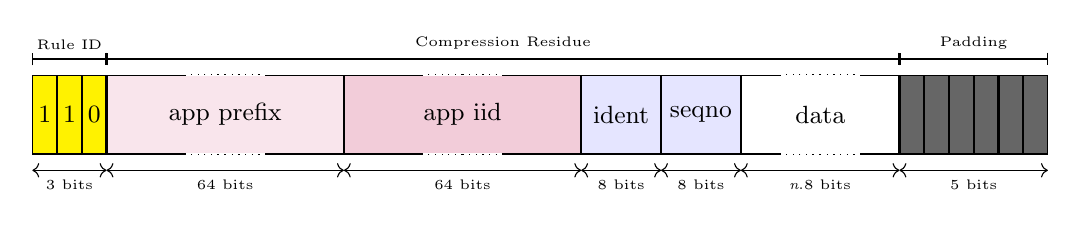
\begin{tikzpicture}

\draw (0,0) node (b1)  [rectangle, draw, minimum height=1cm, minimum width = 0.3cm, fill=yellow] {};
\draw(b1) node {\small{1}};
\draw (b1.east) node (b2)  [right, rectangle, draw, minimum height=1cm, minimum width = 0.3cm, fill=yellow] {};
\draw(b2) node {\small{1}};
\draw (b2.east) node (b3)  [right,rectangle, draw, minimum height=1cm, minimum width = 0.3cm, fill=yellow] {};
\draw(b3) node {\small{0}};

\path(b1.north) -- +(0, 0.2) coordinate(hlineu);

\draw [|-|] (b1.west |- hlineu) -- coordinate(a) (b3.east |- hlineu) ;
\draw (a) node [above] {\tiny{Rule ID}};

\path(b1.south) -- +(0, -0.2) coordinate(hline);

\draw [<->] (b1.west |- hline) -- coordinate(a) (b3.east |- hline) ;
\draw (a) node [below] {\tiny{3 bits}};


\draw (b3.east) node (pref) [right, rectangle, draw, minimum height=1cm, minimum width=3cm, fill=purple!10]{};

\draw [white, thick] (pref.north) -- +(0.5, 0);
\draw [white, thick] (pref.north) -- +(-0.5, 0);
\draw [dotted] (pref.north) -- +(0.5, 0);
\draw [dotted] (pref.north) -- +(-0.5, 0);

\draw [white, thick] (pref.south) -- +(0.5, 0);
\draw [white, thick] (pref.south) -- +(-0.5, 0);
\draw [dotted] (pref.south) -- +(0.5, 0);
\draw [dotted] (pref.south) -- +(-0.5, 0);

\draw (pref) node {\small{app prefix}};

\path(b1.south) -- +(0, -0.2) coordinate(hline);


\draw (pref.east) node (iid) [right, rectangle, draw, minimum height=1cm, minimum width=3cm, fill=purple!20]{};

\draw [white, thick] (iid.north) -- +(0.5, 0);
\draw [white, thick] (iid.north) -- +(-0.5, 0);
\draw [dotted] (iid.north) -- +(0.5, 0);
\draw [dotted] (iid.north) -- +(-0.5, 0);

\draw [white, thick] (iid.south) -- +(0.5, 0);
\draw [white, thick] (iid.south) -- +(-0.5, 0);
\draw [dotted] (iid.south) -- +(0.5, 0);
\draw [dotted] (iid.south) -- +(-0.5, 0);

\draw (iid) node {\small{app iid}};

\path(b1.south) -- +(0, -0.2) coordinate(hline);

\draw [<->] (pref.west |- hline) -- coordinate(a) (pref.east |- hline) ;
\draw (a) node [below] {\tiny{64 bits}};

\draw [<->] (iid.west |- hline) -- coordinate(a) (iid.east |- hline) ;
\draw (a) node [below] {\tiny{64 bits}};

\draw (iid.east) node (ident) [right, rectangle, draw, minimum height=1cm, minimum width=1cm, fill=blue!10]{};
\draw (ident.text) node {\small{ident}};

\draw [<->] (ident.west |- hline) -- coordinate(a) (ident.east |- hline) ;
\draw (a) node [below] {\tiny{8 bits}};

\draw (ident.east) node (seqno) [right, rectangle, draw, minimum height=1cm, minimum width=1cm, fill=blue!10]{};
\draw (seqno.text) node {\small{seqno}};

\draw [<->] (seqno.west |- hline) -- coordinate(a) (seqno.east |- hline) ;
\draw (a) node [below] {\tiny{8 bits}};

\draw (seqno.east) node (data) [right, rectangle, draw, minimum height=1cm, minimum width=2cm]{};
\draw (data.text) node {\small{data}};

\draw [white, thick] (data.north) -- +(0.5, 0);
\draw [white, thick] (data.north) -- +(-0.5, 0);
\draw [dotted] (data.north) -- +(0.5, 0);
\draw [dotted] (data.north) -- +(-0.5, 0);

\draw [white, thick] (data.south) -- +(0.5, 0);
\draw [white, thick] (data.south) -- +(-0.5, 0);
\draw [dotted] (data.south) -- +(0.5, 0);
\draw [dotted] (data.south) -- +(-0.5, 0);

\draw [<->] (data.west |- hline) -- coordinate(a) (data.east |- hline) ;
\draw (a) node [below] {\tiny{\textit{n}.8 bits}};

\draw (data.east) node (p1)  [right, rectangle, draw, minimum height=1cm, minimum width = 0.3cm, fill=black!60] {};
\draw (p1.east) node (p2)  [right, rectangle, draw, minimum height=1cm, minimum width = 0.3cm, fill=black!60] {};
\draw (p2.east) node (p3)  [right,rectangle, draw, minimum height=1cm, minimum width = 0.3cm, fill=black!60] {};
\draw (p3.east) node (p4)  [right,rectangle, draw, minimum height=1cm, minimum width = 0.3cm, fill=black!60] {};
\draw (p4.east) node (p5)  [right,rectangle, draw, minimum height=1cm, minimum width = 0.3cm, fill=black!60] {};
\draw (p5.east) node (p6)  [right,rectangle, draw, minimum height=1cm, minimum width = 0.3cm, fill=black!60] {};

\draw [|-|] (p1.west |- hlineu) -- coordinate(a) (p6.east |- hlineu) ;
\draw (a) node [above] {\tiny{Padding}};

\draw [<->] (p1.west |- hline) -- coordinate(a) (p6.east |- hline) ;
\draw (a) node [below] {\tiny{5 bits}};

\draw [|-|] (b3.east |- hlineu) -- coordinate(a) (p1.west |- hlineu) ;
\draw (a) node [above] {\tiny{Compression Residue}};


\end{tikzpicture}
\caption{ICMPv6 Compression Residue} 
\label{fig-residue} 
\end{figure} 

The rule ID takes 3 bits, followed by the compression residues, the ICMPv6 payload and some padding bits. Since the Rule ID length is 3 bit long and the rest is byte aligned, 5 bits are needed to align the SCHC packet on a  L2-word (i.e. 1 byte).

\section {Compression process}

In OpenSCHC, SCHC Compresssion/Decompression (CD) and Frgamentation/Reassembly (FR) processes are done by the SCHC Machine.

\begin{figure}[!ht] 
\centering 


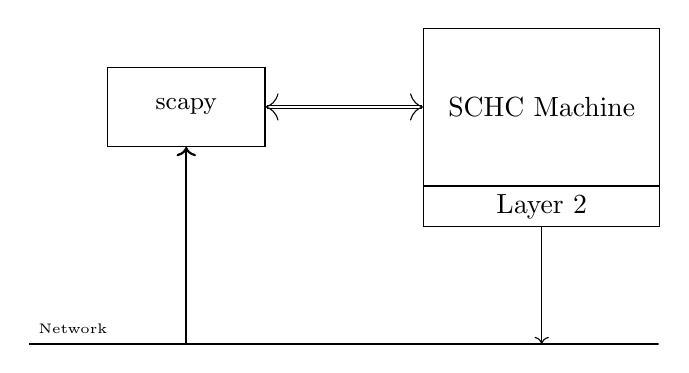
\begin{tikzpicture}

\draw (0,0) node (scapy) [rectangle, draw, minimum width=2cm, minimum height=1cm] {};

\draw (scapy) node {\small{scapy}};

\draw [<-] [thick] (scapy.south) -- coordinate(d) +(0, -2.5) coordinate (a);
\draw [thick] (a) -- +(6, 0) -- +(-2, 0) coordinate (b);

\draw(b) node [above right] {\tiny{Network}};

\draw [<->, double] (scapy.east) -- +(2, 0) coordinate (c);

\draw (c) node (SCHC) [right, rectangle, draw, minimum width=3cm, minimum height=2cm] {};
\draw (SCHC) node {SCHC Machine};
\draw (SCHC.south) node (L2)  [below, rectangle, draw, minimum width = 3cm, minimum height=0.5cm] {};
\draw (L2) node {Layer 2};

\draw [->] (L2.south) -- (L2.south |-a);


\end{tikzpicture}

\caption{Ping gateway architecture} 
\label{fig-schc-archi} 
\end{figure} 

Figure~\vref{fig-schc-archi} gives the architecture of the ping gateway. 
Scapy \textit{sniff} function gets traffic on the network. 
This traffic is composed of IPv6 packets that could be compressed and tunneled SCHC packets that are decompressed. 

\subsection{The code}
\label{sec:compr_code}

The scapy module calls the SCHC Machine, in charge of CD-FR processes. Layer 2 allows to send decompressed packet or a SCHC packet on the network. 

~~
\begin{lstlisting}[language=Python, basicstyle=\ttfamily\scriptsize, caption={Program ping\_core1.py}, label=prog-ping-core1]
import sys
# insert at 1, 0 is the script path (or '' in REPL)
sys.path.insert(1, '../../src/')

from scapy.all import *

import gen_rulemanager as RM
from protocol import SCHCProtocol
from scapy_connection import *
from gen_utils import dprint, sanitize_value

import pprint
import binascii
import socket
import ipaddress


# Create a Rule Manager and upload the rules.
rm = RM.RuleManager()
rm.Add(file="icmp1.json")
rm.Print()

def processPkt(pkt):
    """ called when scapy receives a packet, since this function takes only 
    one argument, schc_machine and scheduler must be specified as a global variable.
    """

    scheduler.run(session=schc_machine)

    # look for a tunneled SCHC pkt
    if pkt.getlayer(Ether) != None: #HE tunnel do not have Ethernet
        e_type = pkt.getlayer(Ether).type
        if e_type == 0x0800:
            ip_proto = pkt.getlayer(IP).proto
            if ip_proto == 17:
                udp_dport = pkt.getlayer(UDP).dport
                if udp_dport == socket_port: # tunnel SCHC msg to be decompressed
                    print ("tunneled SCHC msg")                    
                    schc_pkt, addr = tunnel.recvfrom(2000)
                    other_end = "udp:"+addr[0]+":"+str(addr[1])
                    print("other end =", other_end)
                    r = schc_machine.schc_recv(other_end, schc_pkt)
                    print (r)
            elif ip_proto==41:
                schc_machine.schc_send(bytes(pkt)[34:])

# Start SCHC Machine
POSITION = T_POSITION_CORE

socket_port = 0x5C4C
tunnel = socket.socket(socket.AF_INET, socket.SOCK_DGRAM)
tunnel.bind(("0.0.0.0", socket_port))

lower_layer = ScapyLowerLayer(position=POSITION, socket=tunnel, other_end=None)
system = ScapySystem()
scheduler = system.get_scheduler()
schc_machine = SCHCProtocol(
    system=system,           # define the scheduler
    layer2=lower_layer,      # how to send messages
    role=POSITION,            # DEVICE or CORE
    verbose = True)           
schc_machine.set_rulemanager(rm)

sniff(prn=processPkt, iface="ens3") # scappy cannot read multiple interfaces

\end{lstlisting}

This program~\vref{prog-ping-core1} shows how to compress ICMPv6 packets and send them on a UDP tunnel to a device. It starts with the modules importation from scapy, openSCHC and some regular python modules. Note the importation of the \texttt{scapy\_connection} module, located on the working directory. This module implements the scheduler and the methods to send packets.

\begin{lstlisting}[caption={rule icmp1.json}, backgroundcolor=\color{yellow}, label=rule-icmp1, basicstyle=\ttfamily\tiny],
{
    "DeviceID" : "udp:83.199.24.39:8888",
    "SoR" : [
	 {
	    "RuleID": 6,
	    "RuleIDLength": 3,
	    "Compression": [
		{"FID": "IPV6.VER", "TV": 6, "MO": "equal", "CDA": "not-sent"},
		{"FID": "IPV6.TC",  "TV": 0, "MO": "equal", "CDA": "not-sent"},
		{"FID": "IPV6.FL",  "TV": 0, "MO": "ignore","CDA": "not-sent"},
		{"FID": "IPV6.LEN",          "MO": "ignore","CDA": "compute-length"},
		{"FID": "IPV6.NXT", "TV": 58, "MO": "equal", "CDA": "not-sent"},
		{"FID": "IPV6.HOP_LMT", "TV" : 255,"MO": "ignore","CDA": "not-sent"},
		{"FID": "IPV6.DEV_PREFIX","TV": "2001:470:1F21:1D2::/64",
                                               "MO": "equal","CDA": "not-sent"},
		{"FID": "IPV6.DEV_IID", "TV": "::1","MO": "equal","CDA": "not-sent"},
		{"FID": "IPV6.APP_PREFIX",         "MO": "ignore","CDA": "value-sent"},
		{"FID": "IPV6.APP_IID",         "MO": "ignore","CDA": "value-sent"},
		{"FID": "ICMPV6.TYPE",  "DI": "DW", "TV": 128,"MO": "equal","CDA": "not-sent"},
		{"FID": "ICMPV6.TYPE",  "DI": "UP", "TV": 129,"MO": "equal","CDA": "not-sent"},
		{"FID": "ICMPV6.CODE",  "TV": 0,  "MO": "equal","CDA": "not-sent"},
		{"FID": "ICMPV6.CKSUM", "TV": 0, "MO": "ignore","CDA": "compute-checksum"},
		{"FID": "ICMPV6.IDENT", "TV": 0,"MO": "ignore","CDA": "value-sent"},
		{"FID": "ICMPV6.SEQNO", "TV": 0,"MO": "ignore","CDA": "value-sent"}
		
	    ]
	 },{
		"RuleID" : 12,
		"RuleIDLength" : 11,
		"Fragmentation" : {
			"FRMode": "NoAck",
			"FRDirection": "DW"
		}
	} 
    ]
  }
\end{lstlisting}

~~

The compression process starts with the creation of a Rule Manager \texttt{rm} to include the rules from file \texttt{icmp.json} (cf.~\vref{rule-icmp1}), which contains  the compression rulse we saw below and a NoAck fragmentation rule.

~~

Program continues with the definition of the \texttt{processPkt} function, we will detail after.

~~

The position of the SCHC instance has to be specified. In our example, we are located in the core. The default port number is \texttt{0x5C4C}, the core SCHC instance will wait incoming tunneled SCHC packet on that port.

~~~

Then the SCHC machine is defined. A \texttt{lower\_layer} is created to be used by the SCHC machine when SCHC packet will have to be sent, and a \texttt{system} is created to manage events. From that \texttt{system} a reference to the \texttt{scheduler} is extracted to be used in the \texttt{processPkt} function as a global variable. Then the \texttt{schc\_machine} is created and the previously created rule manager is associated to it.

~~~

Finally, the scapy \texttt{sniff} function is called. The \texttt{processPkt} function is called each time a packet is received on interface \texttt{ens3}\footnote{Scapy allowed to listen simultaneously to several interfaced, for example \texttt{["ens3", "he-ipv6"]}, but since this feature returns sometime some errors, we prefer to listen only to interface \texttt{"ens3"} which will carried tunneled IPv6 packets from Hurricane Electrics.}.

~~~

The \texttt{processPkt} function starts by calling the SCHC machine and then analyses the received packets\footnote{This function must be called regularely, which is the case when some traffic occurs in the network, so it is important not to filter too much incoming traffic.}. 

The functions looks for two types of packets, SCHC tunneled packets coming from devices and IPv6 tunneled packets from Hurricane Electric. The latter are easily recognisable through the use of IP proto 41. When such packet is received, the first 34 bytes corresponding to the Ethernet and IPv4 headers are removed, and the resulting IPv6 packet is send to the SCHC machine for compression.

\subsection{The execution}

Start the program, is sudo mode:

\begin{lstlisting}
$ sudo python3.9 ping_core1.py 
\end{lstlisting}

The program will display the rules and cursor spins, indicating the SCHC machine is running\footnote{The number of received packets determines the spinning speed. It takes 10 packets to change the cursor appearance.}. 

Start pinging the device defined in the rule, the \texttt{-c 1} limits the number of ping messages. 

\begin{lstlisting}
$ ping6 2001:470:1f21:1d2::1 -c 1
\end{lstlisting}

Of course there is no answer to the ping, the openSCHC core instance displays some messages. They can be avoided, if the \texttt{verbose} argument is set to False or not specified when creating the \texttt{schc\_machine} object. 

\begin{lstlisting}[basicstyle=\ttfamily\tiny]
schc recv-from-l3 None None b'`\x05\x0c\x00\x00\x10:8*\x01\xcb\x08\x90:\xbd\x00I\xe0\xa3\xec\x01Vv\x9c \x01\x04p...'
schc parser {('IPV6.VER', 1): [6, 4], ('IPV6.TC', 1): [0, 8], ('IPV6.FL', 1): [330752, 20]...} 
schc compression rule {'RuleID': 6, 'RuleIDLength': 3, 'Compression': [{'FID': 'IPV6.VER', 'FL': 4, ...}
schc compression result b'\xc5\x40\x39\x61\x12\x07\x57\xa0\x09\x3c\x14\x7d\x80\x2a\xce...'/227
schc fragmentation not needed size=227
\end{lstlisting}
 
The openSCHC compression is divided into several steps:
\begin{itemize}
\item Parse the packet; from a sequence of byte received on the network, create a list of fields containing the field identification and their associated value.
\item Find a valid compression rule; ask the rule manager to find a rule matching the parsed packet. The rule selection will also provide the device ID.
\item Apply the compression rule.
\item Send the SCHC packet to the device ID.
\end{itemize}

The first line (\texttt{recv-from-l3}) dumps the original IPv6 packet received by the compressor, corresponding in hexadecimal to:

\begin{lstlisting}[basicstyle=\ttfamily\tiny]
60050c0000103a382a01cb08903abd0049e0a3ec0156769c200104701f2101d20000000000000001800051fb48b20000609f882600060ed2
\end{lstlisting}

~  

The second line (\texttt{parser}) shows three elements returned by the parser. The first one is the list of fields, the second one is the data following the list of fields and the third one is a status code.

The parsed headers are displayed figure:

\begin{lstlisting}[caption={Header Fields of an ICMPv6 message}, label=fig-icmpv6-fields]
{('ICMPV6.CKSUM', 1): [20987, 16],
 ('ICMPV6.CODE', 1): [0, 8],
 ('ICMPV6.IDENT', 1): [18610, 16],
 ('ICMPV6.SEQNO', 1): [0, 16],
 ('ICMPV6.TYPE', 1): [128, 8],
 ('IPV6.APP_IID', 1): [b'I\xe0\xa3\xec\x01Vv\x9c', 64],
 ('IPV6.APP_PREFIX', 1): [b'*\x01\xcb\x08\x90:\xbd\x00', 64],
 ('IPV6.DEV_IID', 1): [b'\x00\x00\x00\x00\x00\x00\x00\x01', 64],
 ('IPV6.DEV_PREFIX', 1): [b' \x01\x04p\x1f!\x01\xd2', 64],
 ('IPV6.FL', 1): [330752, 20],
 ('IPV6.HOP_LMT', 1): [56, 8, 'fixed'],
 ('IPV6.LEN', 1): [16, 16, 'fixed'],
 ('IPV6.NXT', 1): [58, 8, 'fixed'],
 ('IPV6.TC', 1): [0, 8],
 ('IPV6.VER', 1): [6, 4]}
\end{lstlisting}

As shown in figure~\vref{fig-icmpv6-fields}, a header description is a dictionnary where keys are tuple Field ID, position\footnote{In this example, position is always 1 since no field is repeated several time.}, and the value is the tuple field value and value size in bits.

The next element is the data:

\begin{lstlisting}
b'`\x9f\x88&\x00\x06\x0e\xd2'
\end{lstlisting}

and the error code is None.

~~

The third line (\texttt{compression rule}). This no surprise, the rule 6/3 matches. The following listing gives the SCHC packet in hecadecimal:


\begin{lstlisting}
b'c5403961120757a0093c147d802aced3891640000c13f104c000c1da40'
\end{lstlisting}

~~~

The fourth line \texttt{compression result} gives the SCHC packet. Note the \texttt{/227}\footnote {227 \% 8 = 3.  Since the all the residues are byte alligned, the 3 represent the rule ID length. 5 bits of padding will have to be addeed.} at the end, indicating the length in bits. 



~~

No fragmentation is required, so the SCHC packet is directly sent on the tunnel. A frame capture of UDP frame with port 0x5C4C gives:

\begin{lstlisting}[basicstyle=\ttfamily\scriptsize]
>sudo tcpdump -nXi ens3 udp port 0x5C4C
tcpdump: verbose output suppressed, use -v or -vv for full protocol decode
listening on ens3, link-type EN10MB (Ethernet), capture size 262144 bytes
16:41:48.609729 IP 51.91.121.182.23628 > 83.199.24.39.8888: UDP, length 29
	0x0000:  4500 0039 ac95 4000 4011 751f 335b 79b6  E..9..@.@.u.3[y.
	0x0010:  53c7 1827 5c4c 22b8 0025 1936 c540 3961  S..'\L"..%.6.@9a
	0x0020:  1207 57a0 093c 147d 802a ced3 8e5f c000  ..W..<.}.*..._..
	0x0030:  0c13 fbb5 8000 d951 80                   .......Q.

\end{lstlisting}
 
\section{The Decompression Process}

\subsection{Decompression}

Let's do the same operation on the device side. The code is almost the same, the position is changed to \texttt{T\_POSITION\_DEVICE}, the interface name is adapted to its name on the device side.

\begin{lstlisting}[language=Python, caption={Program ping\_device1.py}, label=prog-ping-device1, basicstyle=\ttfamily\scriptsize]
import sys
# insert at 1, 0 is the script path (or '' in REPL)
sys.path.insert(1, '../../src/')

from scapy.all import *

import gen_rulemanager as RM
from protocol import SCHCProtocol
from scapy_connection import *
from gen_utils import dprint, sanitize_value

import pprint
import binascii
import socket
import ipaddress


# Create a Rule Manager and upload the rules.
rm = RM.RuleManager()
rm.Add(file="icmp1.json")
rm.Print()

def processPkt(pkt):
    """ called when scapy receives a packet, since this function takes only one argument,
    schc_machine and scheduler must be specified as a global variable.
    """

    scheduler.run(session=schc_machine)

    # look for a tunneled SCHC pkt
    if pkt.getlayer(Ether) != None: #HE tunnel do not have Ethernet
        e_type = pkt.getlayer(Ether).type
        if e_type == 0x0800:
            ip_proto = pkt.getlayer(IP).proto
            if ip_proto == 17:
                udp_dport = pkt.getlayer(UDP).dport
                if udp_dport == socket_port: # tunnel SCHC msg to be decompressed
                    print ("tunneled SCHC msg")                    
                    schc_pkt, addr = tunnel.recvfrom(2000)
                    r = schc_machine.schc_recv(device_id=device_id, schc_packet=schc_pkt)
                    print (r)
            elif ip_proto==41:
                schc_machine.schc_send(bytes(pkt)[34:])

# Start SCHC Machine
POSITION = T_POSITION_DEVICE

from requests import get

ip = get('https://api.ipify.org').text

socket_port = 8888
tunnel = socket.socket(socket.AF_INET, socket.SOCK_DGRAM)
tunnel.bind(("0.0.0.0", socket_port))

device_id = 'udp:'+ip+":"+str(socket_port)
print ("device_id is", device_id)

lower_layer = ScapyLowerLayer(position=POSITION, socket=tunnel, other_end=None)
system = ScapySystem()
scheduler = system.get_scheduler()
schc_machine = SCHCProtocol(
    system=system,           # define the scheduler
    layer2=lower_layer,      # how to send messages
    role=POSITION,           # DEVICE or CORE
    verbose = True)         
schc_machine.set_rulemanager(rm)

sniff(prn=processPkt, iface="en0") # scappy cannot read multiple interfaces

\end{lstlisting}

 Since the \texttt{device\_id}, in our example, is based on a public IP address, the call to \texttt{https://api.ipify.org} returns the IPv4 public address of the device. 
 
 ~~

In the packet processing, a tunnel is identified. Even, if the scapy buffer, constains the packet, the regular \texttt{recvfrom} socket function is used to recover the data. They are sent to the SCHC machine, which decompress it and returns a field description.

\begin{lstlisting}
{('ICMPV6.CKSUM', 1): ('CCCC', 16),
 ('ICMPV6.CODE', 1): [0, 8],
 ('ICMPV6.IDENT', 1): [31025, 16],
 ('ICMPV6.SEQNO', 1): [8749, 16],
 ('ICMPV6.TYPE', 1): [128, 8],
 ('IPV6.APP_IID', 1): [5323434993581979292, 64],
 ('IPV6.APP_PREFIX', 1): [3026923662209629440, 64],
 ('IPV6.DEV_IID', 1): [b'\x00\x00\x00\x00\x00\x00\x00\x01', 64],
 ('IPV6.DEV_PREFIX', 1): [b' \x01\x04p\x1f!\x01\xd2', 64],
 ('IPV6.FL', 1): [0, 20],
 ('IPV6.HOP_LMT', 1): [255, 8],
 ('IPV6.LEN', 1): ('LLLL', 16),
 ('IPV6.NXT', 1): [58, 8],
 ('IPV6.TC', 1): [0, 8],
 ('IPV6.VER', 1): [6, 4]}
\end{lstlisting}

Note that \texttt{IPV6.LEN} and \texttt{ICMPV6.CKSUM} to, which a \texttt{compute-*} CDA had been associated, contain respectively \texttt{'LLLL'} and \texttt{'CCCC'} values\footnote{In fact, these values will be computed directly by scapy when generating a packet from this field description.}.

\subsection{Device optimization}

In the previous example (cf. listing~\vref{prog-ping-device1}) we started to reconstruct the packet. We can optimize the process on the device. The rule 6/3 (cf. rule figure~\vref{rule-icmp1}) has been associated to the ping traffic. For the downlink, the type is an Echo Request (128) and for the uplink the type is an Echo Reply (129). The other fields remain unchanged in both directions.


~~

Therefore, when the device receives an SCHC packet with rule 6/3, it can send it back to the SCHC core instance to answer with a reply.
We simplify the ping request processing by testing if the rule ID is equal\footnote{Remeber the comparison must be done on the rule ID value and length}.. to the pink6 rule. In that case, the device just echoes the SCHC packet containing the sequence number and identifier, as show in listing figure~\vref{prog-ping-device2}.

\begin{lstlisting}[language=Python, caption={Program ping\_device2.py}, label=prog-ping-device2, basicstyle=\ttfamily\scriptsize]
import sys
# insert at 1, 0 is the script path (or '' in REPL)
sys.path.insert(1, '../../src/')

from scapy.all import *

import gen_rulemanager as RM
from protocol import SCHCProtocol
from scapy_connection import *
from gen_utils import dprint, sanitize_value
from gen_bitarray import *

import pprint
import binascii
import socket
import ipaddress

# Create a Rule Manager and upload the rules.
rm = RM.RuleManager()
rm.Add(file="icmp1.json")
rm.Print()

def processPkt(pkt):
    """ called when scapy receives a packet, since this function takes only one argument,
    schc_machine and scheduler must be specified as a global variable.
    """

    scheduler.run(session=schc_machine)

    # look for a tunneled SCHC pkt
    if pkt.getlayer(Ether) != None: #HE tunnel do not have Ethernet
        e_type = pkt.getlayer(Ether).type
        if e_type == 0x0800:
            ip_proto = pkt.getlayer(IP).proto
            if ip_proto == 17:
                udp_dport = pkt.getlayer(UDP).dport
                if udp_dport == socket_port: # tunnel SCHC msg to be decompressed
                    print ("tunneled SCHC msg")                    
                    schc_pkt, addr = tunnel.recvfrom(2000)
                    schc_bbuf = BitBuffer(schc_pkt)
                    rule = rm.FindRuleFromSCHCpacket(schc=schc_bbuf, device=device_id)
                    if rule[T_RULEID] == 6 and rule[T_RULEIDLENGTH]== 3:
                        print ("ping")
                        tunnel.sendto(schc_pkt, addr)
                    else: 
                        r = schc_machine.schc_recv(device_id=device_id, 
                            schc_packet=schc_pkt)
            elif ip_proto==41:
                schc_machine.schc_send(bytes(pkt)[34:])

# Start SCHC Machine
POSITION = T_POSITION_DEVICE

from requests import get

ip = get('https://api.ipify.org').text

socket_port = 8888
tunnel = socket.socket(socket.AF_INET, socket.SOCK_DGRAM)
tunnel.bind(("0.0.0.0", socket_port))

device_id = 'udp:'+ip+":"+str(socket_port)
print ("device_id is", device_id)

lower_layer = ScapyLowerLayer(position=POSITION, socket=tunnel, other_end=None)
system = ScapySystem()
scheduler = system.get_scheduler()
schc_machine = SCHCProtocol(
    system=system,           # define the scheduler
    layer2=lower_layer,      # how to send messages
    role=POSITION,           # DEVICE or CORE
    verbose = True)         
schc_machine.set_rulemanager(rm)

sniff(prn=processPkt, iface="en0") # scappy cannot read multiple interfaces

\end{lstlisting}

\section{Generating packets}

Now, the SCHC core instance receives SCHC packets from the device, in the tunnel. 
The call to the SCHC machine schc\_recv methods returns the uncompressed packet, which is sent through scapy.

\begin{lstlisting}[language=Python, caption={Program ping\_core2.py}, label=prog-ping-core2, basicstyle=\ttfamily\scriptsize]
import sys
# insert at 1, 0 is the script path (or '' in REPL)
sys.path.insert(1, '../../src/')

from scapy.all import *

import gen_rulemanager as RM
from protocol import SCHCProtocol
from scapy_connection import *
from gen_utils import dprint, sanitize_value

import pprint
import binascii
import socket
import ipaddress


# Create a Rule Manager and upload the rules.
rm = RM.RuleManager()
rm.Add(file="icmp1.json")
rm.Print()

def processPkt(pkt):
    """ called when scapy receives a packet, since this function takes only one argument,
    schc_machine and scheduler must be specified as a global variable.
    """

    scheduler.run(session=schc_machine)

    # look for a tunneled SCHC pkt
    if pkt.getlayer(Ether) != None: #HE tunnel do not have Ethernet
        e_type = pkt.getlayer(Ether).type
        if e_type == 0x0800:
            ip_proto = pkt.getlayer(IP).proto
            if ip_proto == 17:
                udp_dport = pkt.getlayer(UDP).dport
                if udp_dport == socket_port: # tunnel SCHC msg to be decompressed
                    print ("tunneled SCHC msg")                    
                    schc_pkt, addr = tunnel.recvfrom(2000)
                    other_end = "udp:"+addr[0]+":"+str(addr[1])
                    print("other end =", other_end)
                    uncomp_pkt = schc_machine.schc_recv(device_id=other_end,
                                 schc_packet=schc_pkt)
                    uncomp_pkt.show()
                    if uncomp_pkt != None:
                        send(uncomp_pkt, iface="he-ipv6")
            elif ip_proto==41:
                schc_machine.schc_send(bytes(pkt)[34:])

# Start SCHC Machine
POSITION = T_POSITION_CORE

socket_port = 0x5C4C
tunnel = socket.socket(socket.AF_INET, socket.SOCK_DGRAM)
tunnel.bind(("0.0.0.0", socket_port))

lower_layer = ScapyLowerLayer(position=POSITION, socket=tunnel, other_end=None)
system = ScapySystem()
scheduler = system.get_scheduler()
schc_machine = SCHCProtocol(
    system=system,           # define the scheduler
    layer2=lower_layer,      # how to send messages
    role=POSITION,           # DEVICE or CORE
    verbose = False)         
schc_machine.set_rulemanager(rm)

sniff(prn=processPkt, iface="ens3") # scappy cannot read multiple interfaces
\end{lstlisting}

\chapter{Fragmenting Ping6}

In this chapter, in addition to compressing a ping6 request we will fragment it.
For that, we will create a ping6 request that exceeds the maximum L2 MTU allowed for the device:

~

\begin{termc}[backgroundcolor=\color{gray!10}, basicstyle=\ttfamily\small, escapechar=@]
ping6 -c 1 -s 200 2001:470:1f21:1d2::2
\end{termc}

\begin{lstlisting}[language=bash, basicstyle=\ttfamily\tiny, showstringspaces=false]
##[ IPv6 ]##
    version   = 6
    tc        = 0
    fl        = 63154
    plen      = 58
    nh        = ICMPv6
    hlim      = 52
    src       = 2001:41d0:302:2200::13b3
    dst       = 2001:470:1f21:1d2::2
##[ ICMPv6 Echo Request ]##
       type      = Echo Request
       code      = 0
       cksum     = 0xbc64
       id        = 0x260
       seq       = 0x1
       data      = '\\xa5\\xf3\x1cb\x00\x00\x00\x00\x9d\r\x00\x00\x00\x00\x00\x10\x1 1\x12\x13\x14\x15\x16\x17\x18
                    \x19\x1a\x1b\x1c\x1d\x1e\x1f!"#$%&\'()*+,-./0123456789:;<=>?@ABCDEFGHIJKLMNOPQRSTUVWXYZ[\\]^_`
                    abcdefghijklmnopqrstuvwxyz{|}~\x7f\\x80\\x81\\x82\\x83\\x84\\x85\\x86\\x87\\x88\\x89\\x8a\\x8b
                    \\x8c\\x8d\\x8e\\x8f\\x90\\x91\\x92\\x93\\x94\\x95\\x96\\x97\\x98\\x99\\x9a\\x9b\\x9c\\x9d\\x9e
                    \\x9f\\xa0\\xa1\\xa2\\xa3\\xa4\\xa5\\xa6\\xa7\\xa8\\xa9\\xaa\\xab\\xac\\xad\\xae\\xaf\\xb0\\xb1
                    \\xb2\\xb3\\xb4\\xb5\\xb6\\xb7\\xb8\\xb9\\xba\\xbb\\xbc\\xbd\\xbe\\xbf\\xc0\\xc1\\xc2\\xc3\\xc4
                    \\xc5\\xc6\\xc7''

    0000  FA 16 3E E9 DB 5D A2 C8 13 C9 D8 BC 08 00 45 00  ..>..]........E.
    0010  01 0C 79 DB 40 00 F0 29 33 33 D8 42 57 66 33 5B  ..y.@..)33.BWf3[
    0020  79 B6 60 00 F6 B2 00 D0 3A 34 20 01 41 D0 03 02  y.`.....:4 .A...
    0030  22 00 00 00 00 00 00 00 13 B3 20 01 04 70 1F 21  "......... ..p.!
    0040  01 D2 00 00 00 00 00 00 00 02 80 00 88 08 02 6B  ...............k
    0050  00 01 41 00 1D 62 00 00 00 00 14 3B 07 00 00 00  ..A..b.....;....
    0060  00 00 10 11 12 13 14 15 16 17 18 19 1A 1B 1C 1D  ................
    0070  1E 1F 20 21 22 23 24 25 26 27 28 29 2A 2B 2C 2D  .. !"#$%&'()*+,-
    0080  2E 2F 30 31 32 33 34 35 36 37 38 39 3A 3B 3C 3D  ./0123456789:;<=
    0090  3E 3F 40 41 42 43 44 45 46 47 48 49 4A 4B 4C 4D  >?@ABCDEFGHIJKLM
    00a0  4E 4F 50 51 52 53 54 55 56 57 58 59 5A 5B 5C 5D  NOPQRSTUVWXYZ[\]
    00b0  5E 5F 60 61 62 63 64 65 66 67 68 69 6A 6B 6C 6D  ^_`abcdefghijklm
    00c0  6E 6F 70 71 72 73 74 75 76 77 78 79 7A 7B 7C 7D  nopqrstuvwxyz{|}
    00d0  7E 7F 80 81 82 83 84 85 86 87 88 89 8A 8B 8C 8D  ~...............
    00e0  8E 8F 90 91 92 93 94 95 96 97 98 99 9A 9B 9C 9D  ................
    00f0  9E 9F A0 A1 A2 A3 A4 A5 A6 A7 A8 A9 AA AB AC AD  ................
    0100  AE AF B0 B1 B2 B3 B4 B5 B6 B7 B8 B9 BA BB BC BD  ................
    0110  BE BF C0 C1 C2 C3 C4 C5 C6 C7                    ..........
\end{lstlisting}

As one may notice, in this case the size of the \texttt{data} field of the ICMPv6 Echo Request is expanded in order to make the total package size larger. 
In this way, when the query arrives at the core it has to be first compressed and then fragmented so that it conforms to the MTU accepted by the device.

~

The following fragmentation rules are then added to the SoR and can be applied to that traffic:

\begin{lstlisting}[caption={Fragmentation Rules in rule icmp2.json}, backgroundcolor=\color{yellow}, basicstyle=\ttfamily\small, label=rule-icmp2]
	 },{
		"RuleID" : 12,
		"RuleIDLength" : 11,
		"Fragmentation" : {
			"FRMode": "NoAck",
			"FRDirection": "DW"
	 }
	 },{	
		"RuleID" : 13,
		"RuleIDLength" : 11,
		"Fragmentation" : {
		"FRMode": "NoAck",
		"FRDirection": "UP"
		} 
    }
]
}
\end{lstlisting}

\section{Understanding fragmentation rules}

In addition to the rule ID, the rule ID length a fragmentation rule contains two  parameters: the mode and the direction.

~

In order to support reliability, variable L2 MTUs and unidirectional links, the RFC 8724 defines three different fragmentation modes: (i) No-Ack, designed for limited and variable MTU sizes under the assumption that there is no out-of-sequence delivery, (ii) Ack-on-Error for variable MTU and out-of-order delivery using sporadic ACK messages and (iii) Ack-allways for invariable MTUs and no out-of-sequence delivery.
In the following we will go deeper into details of these three modes.

~

As for the direction, it is necessary to stay the behaviour of the SCHC action based on where the traffic is originated.
In our example, we will use the rule \texttt{12/11} for fragmentation on Downlink and rule \texttt{13/11} for fragmentation on Uplink.
Therefore, if the traffic goes from the core to the device (Downlink), we use rule \texttt{12/11} for fragmenting the traffic at the core side and reassembling at the device side.
On the contrary, rule \texttt{13/11} is used for fragmenting the traffic going from the device to the co and for the reassembly processes at the core side.

~

As stated in RFC 8724, in OpenSCHC, SCHC Fragmentation is always done after compression\footnote{It shall rather be noted that, the no-compression rule is also permitted. Therefore, if one is willing to use only SCHC Fragmentation, two rules should be defined: (i) no-compression rule and (ii) the desired fragmentation rule.}. 
Then, as shown in Figure~\ref{fig:icmpv6_query} the whole process goes as following:

\begin{figure}[!tbp]
  \begin{minipage}[b]{0.33\columnwidth}
  \centering
    \usetikzlibrary{shadows,arrows.meta,positioning,backgrounds,fit}

\usetikzlibrary{shapes}
\usetikzlibrary{shapes.callouts}
\usetikzlibrary{shapes.geometric}

\usetikzlibrary{arrows}
\usetikzlibrary{decorations}
\usetikzlibrary{snakes}
\usetikzlibrary{calc}
\usetikzlibrary{patterns}

\usetikzlibrary{matrix,patterns,chains}
\usetikzlibrary{arrows,automata}
\usetikzlibrary{mindmap,trees}
\usetikzlibrary{shapes,snakes}
\usetikzlibrary{circuits.logic.US}
\usetikzlibrary{calc,intersections}

\tikzset{input/.style=coordinate}
\tikzset{output/.style=coordinate}
\tikzset{
  % coord node style is used for placing corners of connecting lines
  coord/.style={coordinate, on chain, on grid, node distance=6mm and 25mm},
  test/.style={draw, diamond, aspect=2, text width=5em},
  block/.style={draw, rectangle,
  minimum height=3em,
  minimum width=7em}}
  
\tikzset{pinstyle/.style={pin edge={to-,thin,black}}}

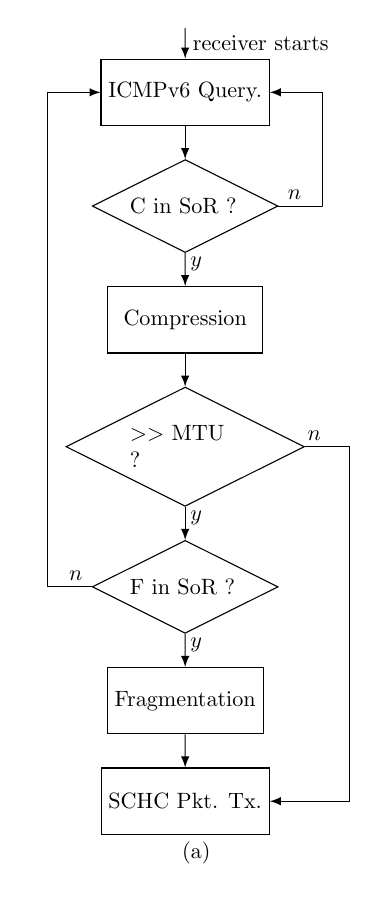
\begin{tikzpicture}[%auto, node distance=2cm,>=latex',
    xscale=0.8,
    yscale=0.8,
    transform shape,
    >=latex,              % Nice arrows; your taste may be different
    start chain=going below,    % General flow is top-to-bottom
    node distance=6mm and 60mm, % Global setup of box spacing
    every join/.style={norm},   % Default linetype for connecting boxes
    ]

\node (input) [input] {\textit{start}};

\node (start) [below right] at (input.south) {receiver starts};

\node (rx) [block, below, align=left] at (start.south west)
{ICMPv6 Query.};

\node (selectc) [test, below, align=left, yshift=-1.5em] at (rx.south)
{C in SoR ?};

\node [coord, right=of selectc] (non)  {}; %coordinates for the non path

\path (selectc.east) to node [near start, yshift = 0.5em] {$n$} (non); 
\path (selectc.south) to node [near start, xshift = 0.5em, yshift = -0.5em] {$y$} (selectc);

\node (comp) [block, below, align=left, yshift=-1.5em] at (selectc.south)
{Compression};

\node (selectmtu) [test, below, align=left, yshift=-1.5em] at (comp.south)
{$>>$ MTU ?};
\node [coord, right=of selectmtu] (non1)  {}; %coordinates for the non path
\path (selectmtu.east) to node [near start, yshift = 0.5em] {$n$} (non1); 
\path (selectmtu.south) to node [near start, xshift = 0.5em, yshift = -0.5em] {$y$} (selectmtu);

\node (selectf) [test, below, align=left, yshift=-1.5em] at (selectmtu.south)
{F in SoR ?};

\node [coord, left=of selectf] (non2)  {}; %coordinates for the non path
\path (selectf.west) to node [near start, yshift = 0.5em] {$n$} (non2); 
\path (selectf.south) to node [near start, xshift = 0.5em, yshift = -0.5em] {$y$} (selectf);


\node (frag) [block, below, align=left, yshift=-1.5em] at (selectf.south)
{Fragmentation};

\node (tx) [block, below, align=left, yshift=-1.5em] at (frag.south)
{SCHC Pkt. Tx.};

\draw [->] (input) --  (rx);    
\draw [->] (rx.south) -- (selectc);
\draw [->] (selectc.south) --  (comp);
\draw [->] (comp.south) --  (selectmtu);
\draw [->] (selectmtu.south) --  (selectf);
\draw [->] (selectf.south) --  (frag);
\draw [->] (frag.south) --  (tx);

\coordinate (fb) at ($(selectc.east)+(2em,0)$); %fb -- feedback
\draw [->] (selectc.east) -| (fb) |- (rx.east);

\coordinate (fb1) at ($(selectf.west)-(2em,0)$); %fb -- feedback
\draw [->] (selectf.west) -| (fb1) |- (rx.west);

\coordinate (fb) at ($(selectmtu.east)+(2em,0)$); %fb -- feedback
\draw [->] (selectmtu.east) -| (fb) |- (tx.east);

\path (tx.south) to node [near start, xshift = 0.5em, yshift = -0.8em] {(a)} (tx);


%\coordinate (fb) at ($(jam.west)+(-2em,0)$); %fb -- feedback
%\draw [->] (output) -| (fb) |- (loop.west);
%\coordinate (fb1) at ($(select.east)+(2em,0)$); %fb -- feedback
%\draw [->] (select.east) -| (fb1) |- (loop.east);

%\node (label) [below, yshift = - 0.3em] at (jam.south) {(a)};

\end{tikzpicture}
  \end{minipage}
  \hfill
  \begin{minipage}[b]{0.33\columnwidth}
  \centering
    \usetikzlibrary{shadows,arrows.meta,positioning,backgrounds,fit}

\usetikzlibrary{shapes}
\usetikzlibrary{shapes.callouts}
\usetikzlibrary{shapes.geometric}

\usetikzlibrary{arrows}
\usetikzlibrary{decorations}
\usetikzlibrary{snakes}
\usetikzlibrary{calc}
\usetikzlibrary{patterns}

\usetikzlibrary{matrix,patterns,chains}
\usetikzlibrary{arrows,automata}
\usetikzlibrary{mindmap,trees}
\usetikzlibrary{shapes,snakes}
\usetikzlibrary{circuits.logic.US}
\usetikzlibrary{calc,intersections}


\tikzset{input/.style=coordinate}
\tikzset{output/.style=coordinate}
\tikzset{
  % coord node style is used for placing corners of connecting lines
  coord/.style={coordinate, on chain, on grid, node distance=6mm and 25mm},
  test/.style={draw, diamond, aspect=2, text width=5em},
  block/.style={draw, rectangle,
  minimum height=3em,
  minimum width=7em}}
  
\tikzset{pinstyle/.style={pin edge={to-,thin,black}}}

\begin{tikzpicture}[%auto, node distance=2cm,>=latex',
    xscale=0.8,
    yscale=0.8,
    transform shape,
    >=latex,              % Nice arrows; your taste may be different
    %start chain=1 going right,    % General flow is top-to-bottom
    node distance=6mm and 60mm, % Global setup of box spacing
    every join/.style={norm},   % Default linetype for connecting boxes
    ]



\node (input) [input] {\textit{start}};

\node (start) [below right] at (input.south) {transmitter starts};

\node (rx) [block, below, align=left] at (start.south west)
{SCHC Pkt Rx.};

\node (selectf) [test, below, align=left, yshift=-1.5em] at (rx.south)
{F in SoR ?};

\node [coord, right=of selectf] (non)  {}; %coordinates for the non path

\path (selectf.west) to node [near start, yshift = 0.5em, xshift = -3em] {$n$} (non); 
\path (selectf.south) to node [near start, xshift = 0.5em, yshift = -0.5em] {$y$} (selectf);

\node (reas) [block, below, align=left, yshift=-1.5em] at (selectf.south)
{Reassembly};

\node (selectc) [test, below, align=left, yshift=-1.5em] at (reas.south)
{C in SoR ?};
\node [coord, right=of selectc] (non)  {}; %coordinates for the non path
\path (selectc.east) to node [near start, yshift = 0.5em] {$n$} (non1); 
\path (selectc.south) to node [near start, xshift = 0.5em, yshift = -0.5em] {$y$} (selectc);


\node (decomp) [block, below, align=left, yshift=-1.5em] at (selectc.south)
{Decompression};

\node [coord, right=of decomp] (non1)  {}; %coordinates for the non path


\node (query) [block, below, align=left, yshift=-1.5em] at (decomp.south)
{ICMPv6 Query};

\node (resp) [block, below, align=left, yshift=-1.5em] at (query.south)
{Echo App.};

\draw [->] (input) --  (rx);    
\draw [->] (rx.south) -- (selectf);
\draw [->] (selectf.south) --  (reas);
\draw [->] (reas.south) --  (selectc);
\draw [->] (selectc.south) --  (decomp);
\draw [->] (decomp.south) --  (query);
\draw [->] (query.south) --  (resp);

\coordinate (fb) at ($(selectf.west)-(2em,0)$); %fb -- feedback
\draw [->] (selectf.west) -| (fb) |- (selectc.west);

\coordinate (fb1) at ($(selectc.east)+(2em,0)$); %fb -- feedback
\draw [->] (selectc.east) -| (fb1) |- (rx.east);

\node (label) [below, yshift = - 0.3em] at (resp.south) {(b)};

\end{tikzpicture}

  \end{minipage}
\caption{ICMPv6 Query Reception when MTU exceeds L2 MTU: (a) Receiver behaviour, (b) Transmitter behaviour.}    \label{fig:icmpv6_query}
\end{figure}

\begin{itemize}
    \item ICMPv6 Echo Request Query Reception at core (Figure.\ref{fig:icmpv6_query}(a))
\begin{enumerate}
    \item An user send a ICMPv6 Echo request exceeding the maximum MTU allowed.
    \item The request arrives at the core side. It verifies if there is a compression rule on its SoR applicable to this specific traffic.
    \item If it exists, the core applies the compression rule. 
    Then, it verifies if the resulting packet surpasses the L2 MTU size.
    \item If yes, the core verifies if there is a fragmentation rule on dowlink.
    \item If there is one, the core applies the fragmentation using the mode defined in the rule.
    \item The core starts to send fragments to the device.
    \end{enumerate}

\item ICMPv6 Echo Request Query Reception at device (Figure.\ref{fig:icmpv6_query}(b)) : 
\begin{enumerate}
    \item The device receives SCHC packets containing the fragments.
    \item The device verifies if there is a fragmentation rule and start the reassembly process.
    \item Once the reassembly process is finished, the device search for a compression ruls applicable to this specific traffic.
    \item The device applies the compression rule to decompress the packet.
    \item The device retrieves the ICMPv6 Echo Reply Query.
    \item At the application level, the device creates a ICMPv6 Echo Reply.
\end{enumerate}

\item ICMPv6 Echo Reply Query Transmission at device (Figure.\ref{fig:icmpv6_query}(a)) : 
\begin{enumerate}
    \item The device verifies if there is a Compression rule for the ICMPv6 Echo Reply.
    \item If yes, the device compress the packet.
    \item The device verifies if the resulting packet surpasses the L2 MTU size.
    \item If yes, it looks for a Fragmentation rule in its SoR applicable to this traffic.
    \item If there is one, the device applies the fragmentation using the mode as defined in the rule.
    \item The device start to send fragments to the device.
\end{enumerate}

\item ICMPv6 Echo Reply Query Reception at core (Figure.\ref{fig:icmpv6_query}(b)) : 
\begin{enumerate}
    \item The core receives SCHC packets containing the fragments.
    \item The core verifies if there is fragmentation rule in its SoR, if yes, it starts the reassembly process.
    \item Once finished, the core search for compression rules applicable to this specific traffic 
    \item If there is a compression rue, it decompress the packet.
    \item The core forwards the ICMPv6 Echo Reply to the user.
\end{enumerate}
\end{itemize}


\section{Fragmentation in No-ACK mode}

This fragmentation mode is designed for no out-of sequence delivery and admits variable L2 MTU.
In No-ACK mode, there is no communication from the fragment receiver to the fragment sender.  
The sender transmits all the SCHC Fragments without expecting any acknowledgement.  
Therefore, there is no need for bidirectional links.

\subsection{SCHC Fragments Format}

In No-ACK, there are two kinds of SCHC Fragments: (i) \texttt{All-0} fragments presented in Figure.\ref{fig:all-0}, and the last fragment called \texttt{All-1} depicted in Figure.\ref{fig:all-1}
An all-0 fragment, is composed of the following fields\footnote{The RFC 8724 also defines the \texttt{DTag} (Datagram Tag) and the \texttt{W} (Window) fields. The former is used for differentiating SCHC F/R messages belonging to different SCHC Packets, for our example this field is not present, and the latter, representing the Window size used in Ack-on-Error and Ack-Allways modes}:

~

\begin{itemize}
    \item \texttt{RuleID}
    %\item W:
    \item \texttt{FCN}: It is used to differentiate All-0 and All-1 fragments. 
    \item \texttt{Fragment Payload}: Corresponds to the payload. Its size is aligned to the remaining space from to fit the L2 MTU.
\end{itemize}

~

\begin{figure}[!ht] 
    \centering 
    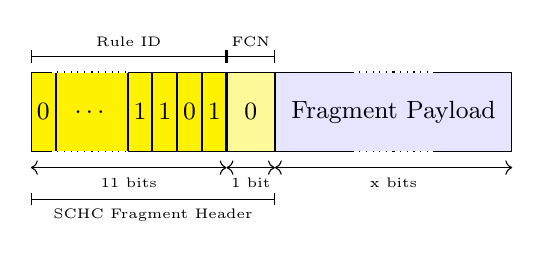
\begin{tikzpicture}

\draw (0,0) node (b1)  [rectangle, draw, minimum height=1cm, minimum width = 0.3cm, fill=yellow] {};
\draw(b1) node {\small{0}};
\draw (b1.east) node (b2)  [right, rectangle, draw, minimum height=1cm, minimum width = 0.9cm, fill=yellow] {};
\draw(b2) node {\small{\dots}};


\draw [white, thick] (b2.north) -- +(0.5, 0);
\draw [white, thick] (b2.north) -- +(-0.5, 0);

\draw [dotted] (b2.north) -- +(0.5, 0);
\draw [dotted] (b2.north) -- +(-0.5, 0);

\draw [white, thick] (b2.south) -- +(0.5, 0);
\draw [white, thick] (b2.south) -- +(-0.5, 0);

\draw [dotted] (b2.south) -- +(0.5, 0);
\draw [dotted] (b2.south) -- +(-0.5, 0);


\draw (b2.east) node (b8)  [right, rectangle, draw, minimum height=1cm, minimum width = 0.3cm, fill=yellow] {};
\draw(b8) node {\small{1}};

\draw (b8.east) node (b9)  [right, rectangle, draw, minimum height=1cm, minimum width = 0.3cm, fill=yellow] {};
\draw(b9) node {\small{1}};

\draw (b9.east) node (b10)  [right, rectangle, draw, minimum height=1cm, minimum width = 0.3cm, fill=yellow] {};
\draw(b10) node {\small{0}};

\draw (b10.east) node (b11)  [right, rectangle, draw, minimum height=1cm, minimum width = 0.3cm, fill=yellow] {};
\draw(b11) node {\small{1}};
\path(b1.north) -- +(0, 0.2) coordinate(hlineu);

\draw [|-|] (b1.west |- hlineu) -- coordinate(a) (b11.east |- hlineu) ;
\draw (a) node [above] {\tiny{Rule ID}};
\path(b1.south) -- +(0, -0.2) coordinate(hline);

\draw [<->] (b1.west |- hline) -- coordinate(a) (b11.east |- hline) ;
\draw (a) node [below] {\tiny{11 bits}};
\draw (b11.east) node (dtag) [right, rectangle, draw, minimum height=1cm, minimum width=1cm, fill=yellow!30]{};
%\draw (dtag) node {\small{DTag}};
%\path(b1.south) -- +(0, -0.2) coordinate(hline);


%\path(b1.south) -- +(0, -0.2) coordinate(hline);
%\draw [<->] (dtag.west |- hline) -- coordinate(a) (dtag.east |- hline) ;
%\draw (a) node [below] {\tiny{T bits}};


\draw (b11.east) node (fcn) [right, rectangle, draw, minimum height=1cm, minimum width=0.6cm, fill=yellow!40]{};
\draw (fcn.text) node {\small{0}};

\draw [|-|] (fcn.west |- hlineu) -- coordinate(a) (fcn.east |- hlineu) ;
\draw (a) node [above] {\tiny{FCN}};
\path(b1.south) -- +(0, -0.2) coordinate(hline);

\draw [<->] (fcn.west |- hline) -- coordinate(a) (fcn.east |- hline) ;
\draw (a) node [below] {\tiny{1 bit}};

%\draw (fcn.east) node (rcs) [right, rectangle, draw, minimum height=1cm, minimum width=1cm, fill=green!10]{};
%\draw (rcs.text) node {\small{RCS}};

%\draw [<->] (rcs.west |- hline) -- coordinate(a) (rcs.east |- hline) ;
%\draw (a) node [below] {\tiny{32 bits}};

\draw (fcn.east) node (fpay) [right, rectangle, draw, minimum height=1cm, minimum width=3cm, fill=blue!10]{};
\draw (fpay.text) node {\small{Fragment Payload}};

\draw [white, thick] (fpay.north) -- +(0.5, 0);
\draw [white, thick] (fpay.north) -- +(-0.5, 0);
\draw [dotted] (fpay.north) -- +(0.5, 0);
\draw [dotted] (fpay.north) -- +(-0.5, 0);

\draw [white, thick] (fpay.south) -- +(0.5, 0);
\draw [white, thick] (fpay.south) -- +(-0.5, 0);
\draw [dotted] (fpay.south) -- +(0.5, 0);
\draw [dotted] (fpay.south) -- +(-0.5, 0);

\draw [<->] (fpay.west |- hline) -- coordinate(a) (fpay.east |- hline) ;
\draw (a) node [below] {\tiny{x bits}};

\path(b1.south) -- +(0, - 0.6) coordinate(hline1);
\draw [|-|] (b1.west |- hline1) -- coordinate(a) (fcn.east |- hline1) ;
coordinate 
\draw (a) node [below] {\tiny{SCHC Fragment Header}};

\end{tikzpicture}
    \caption{All-0 SCHC Fragment in No-Ack mode} 
    \label{fig:all-0} 
\end{figure} 

The second type of fragment is the \texttt{All-1}, it corresponds to the last fragment. As shown in Figure \ref{fig:all-1}, contrary to the \texttt{All-0}, it also contains the RCS field, and it can also contains padding as needed in order to fit the L2 word size.

\begin{figure}[!ht] 
    \centering 
    \input{figs/all-1-NoAck}
    \caption{All-1 SCHC Fragment in No-Ack mode} 
    \label{fig:all-1} 
\end{figure} 
   
In OpenSCHC the Reassembly Check Sequence (RCS) field corresponds to the result of using the CRC32 algorithm, and as recommended by the RFC 8724 it is computed on the full SCHC packet (after reassembly) concatenated with the padding bits.

\subsection{Fragmentation/Reassembly Process}

In this mode, since there are no fragment acknowledgments, the sender creates as many fragments as needed based on the size of the compressed SCHC packet and the L2 MTU.
Figure \ref{fig:NoAck} presents an example where $n$ fragments are needed. 
In this case, the transmitter creates $n-1$ \texttt{All-0} fragments and one \texttt{All-1} with the corresponding RCS field and padding if needed.

\begin{figure}[!ht] 
    \centering 
    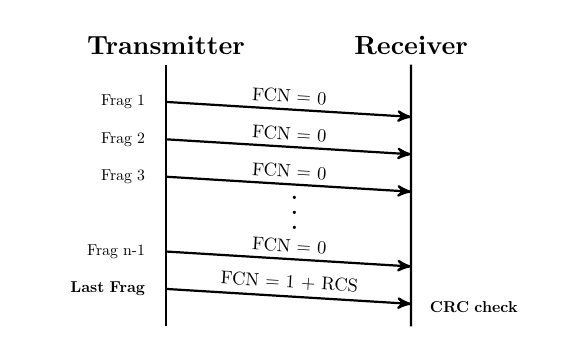
\begin{tikzpicture}[xscale = 0.95, yscale = 0.95,transform shape,>=stealth',thick,
commentl/.style={text width=2.5cm, align=right, scale=.6},
commentr/.style={commentl, align=left}]

\node[] (init) {\textbf{Transmitter}};
\node[right=1.2cm of init] (core) {\textbf{Receiver}};
\node[right=0.4cm of init] (middle) {};

\draw[->] ([yshift=-0.5cm]init.south) coordinate (f1) -- ([yshift=-.2cm]f1-|core)
coordinate (fin1) node[pos=.5, above, sloped, scale=0.7] {FCN = 0};
\node[left = 2mm of f1.west, commentl]{Frag 1};

\draw[->] ([yshift=-1cm]init.south) coordinate (f2) -- ([yshift=-.7cm]f1-|core)
coordinate (fin2) node[pos=.5, above, sloped, scale=0.7] {FCN = 0};
\node[left = 2mm of f2.west, commentl]{Frag 2};

\draw[->] ([yshift=-1.5cm]init.south) coordinate (f3) -- ([yshift=-1.2cm]f1-|core)
coordinate (fin3) node[pos=.5, above, sloped, scale=0.7] {FCN = 0};
\node[left = 2mm of f3.west, commentl]{Frag 3};

\draw[->] ([yshift=-2.5cm]init.south) coordinate (f4) -- ([yshift=-2.2cm]f1-|core)
coordinate (fin4) node[pos=.5, above, sloped, scale=0.7] {FCN = 0};
\node[left = 2mm of f4.west, commentl]{Frag n-1};

\draw[->] ([yshift=-3cm]init.south) coordinate (f5) -- ([yshift=-2.7cm]f1-|core)
coordinate (fin5) node[pos=.5, above, sloped, scale=0.7] {FCN = 1 + RCS};
\node[left = 2mm of f5.west, commentl]{\textbf{Last Frag}};

\node[right = 3.45cm of f5.east, commentr, yshift=-0.4cm]{\textbf{CRC check}};


% dots

\node[scale=0.8] at ([yshift=-1.9cm]middle.south)  {\textbf{.}};
\node[scale=0.8] at ([yshift=-2.1cm]middle.south)  {\textbf{.}};
\node[scale=0.8] at ([yshift=-2.3cm]middle.south)  {\textbf{.}};

%% vertical dotted time-out
%\draw[dotted] ([yshift=-0.5cm]init.255)--([yshift=-0.1cm]init.255|-ack1e);
% Texts
%\node[left = 2mm of f1.west, commentl]{\textbf{SEND FRAG 1}};%\\[-1mm]{\itshape start time-out}};
%\node[left = 2mm of ack1e.west, yshift=-.3cm, commentl]{{\itshape end time-out}\\ \textbf{ACK 1 \\ RECEIVED}};
%\node[right = 2mm of fin1e.west, commentr]{\textbf{MSG 1 \\ RECEIVED}\\[-1mm]{\itshape sending ACK}};

\node[scale=0.8] at (0, -2.7cm) (a) {};
% Drawing vertical time lines 
\draw[thick, shorten >=-1cm] (init) -- (init|-a);
\draw[thick, shorten >=-1cm] (core) -- (core|-a);

\end{tikzpicture}

    \caption{All-1 SCHC Fragment in No-Ack mode} 
    \label{fig:NoAck} 
\end{figure} 

\subsection{The code}

In this section, we will present the code necessary to process an icmpv6 echo request that exceeds the L2 MTU size. 
Two blocks of code are required: core and device programs. 
For the downlink, they are in charge of: 

\begin{itemize}
\item core program: receiving the IPv6 packet, compressing it, fragmenting it and sending the SCHC fragments.
\item device program: reassembling and decompressing SCHC packets and, creating the echo reply packet.
\end{itemize} 

For the uplink, they are in charge of: 

\begin{itemize}
\item device program: compressing and fragmenting the IPv6 Echo Reply packet, and sending the SCHC fragments to the core.
\item core program: reassembling and decompressing SCHC packets and, forwarding the Echo reply IPv6 Packet to the user.
\end{itemize} 

\subsubsection{Core program}

For this example we will extend the code used in Section~\ref{sec:compr_code}. 
As in the previous case the Compression and Fragmentation process starts with the creation of a Rule Manager \texttt{rm} used to add the rules from the file \texttt{icmp2.json} (cf. \vref{rule-icmp2}), which includes the Rule 3 for compressing and Rules 12 and 13 for fragmenting.

~

As presented in Listing~\vref{prog-ping-core2}, the process follows the same logic as in the compression example. 
The \texttt{processPkt} function filters SCHC packets coming from devices and IPv6 tunneled packets from Hurricane Electric. 

~

As in the C/D only example, the \texttt{processPkt} calls the SCHC Machine and then looks at the received packets. 
There can be two kinds off packets: (i) IPv6 tunneled packets filtered by looking at the IP proto 41 and passed to the SCHC Machine removing the first 34 bytes (Ethernet and IPv4 headers), and (ii) SCHC Packets filtered by looking at the UDP socket port \texttt{0x5C4C}.

~
\input{code/ping_core2.py}
~

The former is used to start the F/D process, IPv6 packets are passed to the SCHC Machine using the \texttt{schc\_send} function. 
This function triggers the SCHC actions: (i)~compression, (ii) fragmentation and finally (iii) SCHC Fragment transmission using the scheduler.
And the latter starts the R/D process. 
In such case the \texttt{schc\_recv} triggers the SCHC Actions: (i) Reassembly and (ii) Decompression. This function returns $None$ when it is not the last fragment (All-0) or the decompressed packet when the last fragment arrives.

\subsubsection{Device program}

For the device side, as we can see in \vref{prog-ping-device2}, the code is almost the same, as in the C/D example the position is changed to \texttt{T\_POSITION\_DEVICE} when defining the Rule Manager, this will be used to select the correct rules and CDA.

~

Contrary to the previous example, where the device simply echoes the SCHC packet to the core. 
Here, we use scapy to create the ICMPv6 Echo Reply packet.
Then, this packet is injected into the SCHC Machine by using the \texttt{schc\_send} function.


\input{code/ping_device2.py}

\subsection{The execution}

Start the device and core programs, is sudo mode:

\begin{lstlisting}
$ sudo python3.9 ping_core2.py 
\end{lstlisting}

\begin{lstlisting}
$ sudo python3.9 ping_device2.py 
\end{lstlisting}

The program will display the rules and cursor spins, indicating the SCHC machine is running.
As we can see, three rules are defined: Rule 6/3 for compression, Rule 12/11 for fragmentation in Uplink using No-Ack mode and Rule 13/11 using No-Ack mode.

~

\begin{lstlisting}[basicstyle=\ttfamily\scriptsize, numbers=none]
****************************************
Device: udp:54.37.158.10:8888
/-------------------------\
|Rule 6/3            110  |
|---------------+---+--+--+------------------------------+-------------+----------------\
|IPV6.VER       |  4| 1|BI|                             6|EQUAL        |NOT-SENT        |
|IPV6.TC        |  8| 1|BI|                             0|EQUAL        |NOT-SENT        |
|IPV6.FL        | 20| 1|BI|                             0|IGNORE       |NOT-SENT        |
|IPV6.LEN       | 16| 1|BI|------------------------------|IGNORE       |COMPUTE-LENGTH  |
|IPV6.NXT       |  8| 1|BI|                            58|EQUAL        |NOT-SENT        |
|IPV6.HOP_LMT   |  8| 1|BI|                           255|IGNORE       |NOT-SENT        |
|IPV6.DEV_PREFIX| 64| 1|BI|              200104701f2101d2|EQUAL        |NOT-SENT        |
|IPV6.DEV_IID   | 64| 1|BI|              0000000000000002|EQUAL        |NOT-SENT        |
|IPV6.APP_PREFIX| 64| 1|BI|------------------------------|IGNORE       |VALUE-SENT      |
|IPV6.APP_IID   | 64| 1|BI|------------------------------|IGNORE       |VALUE-SENT      |
|ICMPV6.TYPE    |  8| 1|DW|                           128|EQUAL        |NOT-SENT        |
|ICMPV6.TYPE    |  8| 1|UP|                           129|EQUAL        |NOT-SENT        |
|ICMPV6.CODE    |  8| 1|BI|                             0|EQUAL        |NOT-SENT        |
|ICMPV6.CKSUM   | 16| 1|BI|                             0|IGNORE       |COMPUTE-CHECKSUM|
|ICMPV6.IDENT   | 16| 1|BI|                             0|IGNORE       |VALUE-SENT      |
|ICMPV6.SEQNO   | 16| 1|BI|                             0|IGNORE       |VALUE-SENT      |
\---------------+---+--+--+------------------------------+-------------+----------------/
/-------------------------\
|Rule 12/11     00001100  |
!=========================+=============================================================\
!v Fragmentation mode : NoAck    header dtag 2 Window  0 FCN  3                     DW v!
!v No Tile size specified                                                              v!
!v RCS Algorithm: crc32                                                                v!
\=======================================================================================/
/-------------------------\
|Rule 13/11     00001101  |
!=========================+=============================================================\
!^ Fragmentation mode : NoAck    header dtag 2 Window  0 FCN  3                     UP ^!
!^ No Tile size specified                                                              ^!
!^ RCS Algorithm: crc32                                                                ^!
\=======================================================================================/
/
\end{lstlisting}

Then, we start pinging the device defined in the SoR, the \texttt{-c 1} limits the number of ping messages, and \texttt{-s 50} increases the size of the ICMPv6 packet.

\begin{lstlisting}
$ ping6 -c 1 -s 50 dev2.openschc.net
\end{lstlisting}

And we get as result:

\begin{lstlisting}[basicstyle=\ttfamily\scriptsize]
58 bytes from 2001:470:1f21:1d2::2 (2001:470:1f21:1d2::2): icmp_seq=1 ttl=239 time=136 ms

--- dev2.openschc.net ping statistics ---
1 packets transmitted, 1 received, 0% packet loss, time 0ms
rtt min/avg/max/mdev = 135.661/135.661/135.661/0.000 ms

\end{lstlisting}

The core instance displays :

\begin{lstlisting}[basicstyle=\ttfamily\tiny, numbers=none]
schc recv-from-l3 None None
schc parser {('IPV6.VER', 1): [6, 4],  ('IPV6.TC', 1): [0, 8],  ('IPV6.FL', 1): [749668, 20], 
            ('IPV6.LEN', 1): [58, 16, 'fixed'], ('IPV6.NXT', 1): [58, 8, 'fixed'], 
            ('IPV6.HOP_LMT', 1): [46, 8, 'fixed'], 
            ('IPV6.APP_PREFIX', 1): [b'*\x01\x0e\n\x01\xa6\x1c\xe0', 64], 
            ('IPV6.APP_IID', 1): [b'\xd6\x0fN\x05\xd1z\x14\xcd', 64], 
            ('IPV6.DEV_PREFIX', 1): [b' \x01\x04p\x1f!\x01\xd2', 64], 
            ('IPV6.DEV_IID', 1): [b'\x00\x00\x00\x00\x00\x00\x00\x02', 64], 
            ('ICMPV6.TYPE', 1): [128, 8], ('ICMPV6.CODE', 1): [0, 8], ('ICMPV6.CKSUM', 1): [26192, 16], 
            ('ICMPV6.IDENT', 1): [2, 16], ('ICMPV6.SEQNO', 1): [1, 16]}

schc compression rule {'RuleID': 6, 'RuleIDLength': 3, 
                        'Compression': [{'FID': 'IPV6.VER', 'FL': 4, 'FP': 1, 'DI': 'BI', 'TV': 6, 'MO': 'EQUAL', 
                        'CDA': 'NOT-SENT'}, ... }

schc compression result b\xc5\x40\x21\xc1\x40\x34\xc3\x9c\x1a\xc1\xe9\xc0\xba\x2f\x42\x99\xa0\x00\x40\x00\x31\x38
                          \x8a\xcc\x40\x00\x00\x00\x0d\x51\x20\xc0\x00\x00\x00\x00\x02\x02\x22\x42\x62\x82\xa2\xc2
                          \xe3\x03\x23\x43\x63\x83\xa3\xc3\xe4\x04\x24\x44\x64\x84\xa4\xc4\xe5\x05\x25\x45\x65\x85
                          \xa5\xc5\xe6\x06\x20/563
                          
schc fragmentation rule {'RuleID': 12, 'RuleIDLength': 11, 'Fragmentation': {'FRDirection': 'DW', 'FRMode': 'NoAck', ...}

MTU =  56

r:12/11 (noA) DTAG=0 W=- FCN=All-0
|---- 25------------->
frag_send.py, args: (bytearray(b'\x01\x80\xc5@!\xc1@4\xc3\x9c\x1a\xc1\xe9\xc0\xba/B\x99\xa0\x00@\x0018\x8a'), 
                    'udp:54.37.158.10:8888', None)

Queue running event -> 1, callback -> send_packet
MTU =  56
r:12/11 (noA) DTAG=0 W=- FCN=All-0
|---- 25------------->
frag_send.py, args: (bytearray(b'\x01\x80\xcc@\x00\x00\x00\rQ \xc0\x00\x00\x00\x00\x02\x02"Bb\x82\xa2\xc2\xe3\x03'), 
                    'udp:54.37.158.10:8888', None)
Queue running event -> 2, callback -> send_frag
Queue running event -> 3, callback -> event_sent_frag
Queue running event -> 4, callback -> send_packet
MTU =  56
r:12/11 (noA) DTAG=0 W=- FCN=All-0
|---- 25------------->
frag_send.py, args: (bytearray(b'\x01\x80#Cc\x83\xa3\xc3\xe4\x04$Dd\x84\xa4\xc4\xe5\x05%Ee\x85\xa5\xc5\xe6'), 
                    'udp:54.37.158.10:8888', None)
frag_send.py, _session_id:  udp:54.37.158.10:8888
Queue running event -> 5, callback -> send_frag
Queue running event -> 6, callback -> event_sent_frag
Queue running event -> 7, callback -> send_packet
MTU =  56
SessionManager: deleted ('udp:54.37.158.10:8888', 12, 11, 0)
MIC Size =  32
r:12/11 (noA) DTAG=0 W=- FCN=All-1
|----  8------------->
frag_send.py, args:  (bytearray(b'\x01\x87x\x10\xdc_\x06 '), 'udp:54.37.158.10:8888', None)
frag_send.py, _session_id:  udp:54.37.158.10:8888
Queue running event -> 8, callback -> send_frag
Queue running event -> 9, callback -> send_packet
tunneled SCHC msg
other end = udp:54.37.158.10:8888
			----------- 25--------->|
New reassembly session created ReassemblerNoAck
frag data
			r:13/11 (noA) DTAG=0 W=- FCN=All-0
CANCEL Inactivity Timer None
[b'\xc5\x40\x21\xc1\x40\x34\xc3\x9c\x1a\xc1\xe9\xc0\xba\x2f\x42\x99\xa0\x00\x40\x00\x31\x38\x8a'/184]
tunneled SCHC msg
other end = udp:54.37.158.10:8888
			----------- 25--------->|
Reassembly session found ReassemblerNoAck
frag data
			r:13/11 (noA) DTAG=0 W=- FCN=All-0
CANCEL Inactivity Timer 10
[b'\xc5\x40\x21\xc1\x40\x34\xc3\x9c\x1a\xc1\xe9\xc0\xba\x2f\x42\x99\xa0\x00\x40\x00\x31\x38\x8a'/184, 
b'\xcc\x40\x00\x00\x00\x0d\x51\x20\xc0\x00\x00\x00\x00\x02\x02\x22\x42\x62\x82\xa2\xc2\xe3\x03'/184]
tunneled SCHC msg
other end = udp:54.37.158.10:8888
			----------- 25--------->|
Reassembly session found ReassemblerNoAck
frag data
			r:13/11 (noA) DTAG=0 W=- FCN=All-0
CANCEL Inactivity Timer 11
[b'\xc5\x40\x21\xc1\x40\x34\xc3\x9c\x1a\xc1\xe9\xc0\xba\x2f\x42\x99\xa0\x00\x40\x00\x31\x38\x8a'/184, 
 b'\xcc\x40\x00\x00\x00\x0d\x51\x20\xc0\x00\x00\x00\x00\x02\x02\x22\x42\x62\x82\xa2\xc2\xe3\x03'/184, 
 b'\x23\x43\x63\x83\xa3\xc3\xe4\x04\x24\x44\x64\x84\xa4\xc4\xe5\x05\x25\x45\x65\x85\xa5\xc5\xe6'/184]
tunneled SCHC msg
other end = udp:54.37.158.10:8888
			-----------  8--------->|
Reassembly session found ReassemblerNoAck
frag data
			r:13/11 (noA) DTAG=0 W=- FCN=All-1
CANCEL Inactivity Timer 12
[b'\xc5\x40\x21\xc1\x40\x34\xc3\x9c\x1a\xc1\xe9\xc0\xba\x2f\x42\x99\xa0\x00\x40\x00\x31\x38\x8a'/184, 
 b'\xcc\x40\x00\x00\x00\x0d\x51\x20\xc0\x00\x00\x00\x00\x02\x02\x22\x42\x62\x82\xa2\xc2\xe3\x03'/184, 
 b'\x23\x43\x63\x83\xa3\xc3\xe4\x04\x24\x44\x64\x84\xa4\xc4\xe5\x05\x25\x45\x65\x85\xa5\xc5\xe6'/184, 
 b'\x06\x20'/16]
----------------------- Final Reassembly -----------------------
ALL1 received
b'c54021c14034c39c1ac1e9c0ba2f4299a000400031388acc400000000d5120c000000000020222426282a2c2e30323436
  383a3c3e40424446484a4c4e50525456585a5c5e60620'
  
SUCCESS: MIC matched. packet bytearray(b'x\x10\xdc_') == result b'x\x10\xdc_'
----------------------- Decompression -----------------------
SessionManager: deleted (None, 13, 11, 0)
###[ IPv6 ]### 
  version   = 6
  tc        = 0
  fl        = 0
  plen      = None
  nh        = ICMPv6
  hlim      = 255
  src       = 2001:470:1f21:1d2::2
  dst       = 2a01:e0a:1a6:1ce0:d60f:4e05:d17a:14cd
###[ ICMPv6 Echo Reply ]### 
     type      = Echo Reply
     code      = 0
     cksum     = None
     id        = 0x2
     seq       = 0x1
     data      = bytearray(b'\x89\xc4Vb\x00\x00\x00\x00j\x89\x06\x00\x00\x00\x00\x00\x10\x11\x12\x13...')

.
Sent 1 packets.
schc recv-from-l3 None None
schc parser {('IPV6.VER', 1): [6, 4], ('IPV6.TC', 1): [0, 8], 
             ('IPV6.FL', 1): [0, 20], ('IPV6.LEN', 1): [58, 16, 'fixed'], 
             ('IPV6.NXT', 1): [58, 8, 'fixed'], ('IPV6.HOP_LMT', 1): [255, 8, 'fixed'],
             ('IPV6.APP_PREFIX', 1): [b' \x01\x04p\x1f!\x01\xd2', 64], 
             ('IPV6.APP_IID', 1): [b'\x00\x00\x00\x00\x00\x00\x00\x02', 64], 
             ('IPV6.DEV_PREFIX', 1): [b'*\x01\x0e\n\x01\xa6\x1c\xe0', 64], 
             ('IPV6.DEV_IID', 1): [b'\xd6\x0fN\x05\xd1z\x14\xcd', 64], 
             ('ICMPV6.TYPE', 1): [129, 8], ('ICMPV6.CODE', 1): [0, 8], 
             ('ICMPV6.CKSUM', 1): [25936, 16], ('ICMPV6.IDENT', 1): [2, 16], 
             ('ICMPV6.SEQNO', 1): [1, 16]} 
             
schc compression rule None
schc no-compression rule None
schc rule for compression/no-compression not found
\
.
Sent 1 packets.
\end{lstlisting}

We can see several steps. 
The following are those corresponding to the C/F Process one the ICMPv6 message arrives to the core instance:

~

\begin{itemize}

\item Parse the packet: from a sequence of bytes received on the network, create a list of fields containing the field identification and their associated value.
\item Find a valid compression rule: ask the rule manager to find a rule matching the
parsed packet. 
The rule selection will also provide the device ID.
\item The Rule Manager finds a Compression rule and the SCHC Machine applies the compression rule.
\item The SCHC Machine verifies if the MTU is below the size of the compressed packet, and if not it looks for a fragmentation rule for this packet. 
\item The Rule Manager finds the Rule 12 that correspond to fragmentation in No-Ack mode
\item The SCHC Machine creates a context used to track the fragmentation session. It corresponds to the Rule ID, the Rule ID length and the dtag. In our example dtag is set to zero.
\item The SCHC Machine starts to create fragments and sent it into the Network. 
In this example, three All-0 fragments and 1 All-1 Fragment are created.
\item Fragments are sent on the UDP tunnel using the corresponding device ID 
\\
\texttt{udp:54.37.158.10:8888}
\end{itemize}

~

Then, once the device has performed the R/D process, created the the echo query response and C/F the prompt shows the following messages:

~

\begin{itemize}
\item Scappy sniffs an udp packet and detects that it comes from the device by looking at the IP and corresponding port: \texttt{other\_end = udp:54.37.158.10:8888}.
\item The SCHC Machine creates a reassembly session using the NoAck mode.
\item The SCHC Machine stores all the fragments until the All-1 is received.
\item The SCHC Machine reassembles the fragments and decompress it.
\item Once decompressed, the received packet is printed using scapy; we can see that it correspond to the ICMP Echo Query Response created by the device.
\item Finally, the core sends the IPv6 packet to the user  
\end{itemize}

~

At the device side we get the following messages:

~

\input{code/result_frag_b}

~

We can tell that, the process follows the following steps:

~

\begin{itemize}
    \item Reception of a SCHC Packet
    \item The SCHC Machine detects that it corresponds to a SCHC Fragment and creates a reassembly session and stores the fragments as they arrive.
    \item Once the All-1 arrives, the SCHC Machine reassembles the packet.
    \item The SCHC Machine validates the CRC.
    \item The Echo Reply is created.
    \item As in the core side, the Rule Manager finds a compression rule, then, the packet is parsed, compressed and fragmented.
    \item Three All-0 and one All-1 SCHC fragments are created and sent back to the core.
\end{itemize}

Finally, sudo tcpdump -nXi ens3 udp port 0x5C4C at the core side. 
As we can see SCHC packets are first sent on the tcp tunnel and


\section{Fragmentation in Ack-on-Error mode}
